\documentclass[12pt]{article}
\usepackage[a4paper, margin=1in, top=1.25in, headheight=50pt, headsep=0.25in]{geometry}
\usepackage{graphicx}
\usepackage{fancyhdr}
\usepackage{hyperref}
\usepackage{listings}
\usepackage{xcolor}
\usepackage{float}
\usepackage{lipsum} % Just for placeholder text

\definecolor{codegreen}{rgb}{0,0.6,0}
\definecolor{codegray}{rgb}{0.5,0.5,0.5}
\definecolor{codepurple}{rgb}{0.58,0,0.82}
\definecolor{backcolour}{rgb}{0.95,0.95,0.92}

\lstdefinestyle{mystyle}{
    backgroundcolor=\color{backcolour},   
    commentstyle=\color{codegreen},
    keywordstyle=\color{magenta},
    numberstyle=\tiny\color{codegray},
    stringstyle=\color{codepurple},
    basicstyle=\ttfamily\footnotesize,
    breakatwhitespace=false,         
    breaklines=true,                 
    captionpos=b,                    
    keepspaces=true,                 
    numbers=left,                    
    numbersep=5pt,                  
    showspaces=false,                
    showstringspaces=false,
    showtabs=false,                  
    tabsize=2
}
\lstset{style=mystyle}

\usepackage[colorlinks=true, linkcolor=blue, urlcolor=blue]{hyperref}
\pagestyle{fancy}
\fancyhf{}
\setlength{\headheight}{50pt} 
\setlength{\headsep}{25pt} 
\renewcommand{\headrulewidth}{2pt} 

\fancyhead[L]{
\includegraphics[width=1cm]{logo.png}} 
\fancyhead[R]{User guide\\INFOB318\\UNamur}
\fancyfoot[C]{\thepage}


\renewcommand{\headrule}{\hbox to\headwidth{\color{black}\leaders\hrule height \headrulewidth\hfill}}


% Cover page setup
\title{
    \vspace{-1in}
    \begin{center}
        
\includegraphics[width=4cm]{logo.png} 
    \end{center}
  
    {\large INFOB318: Projet individuel}\\
    \bigskip
\line(1,0){338} \\ 
    \bigskip
    {\huge \textbf{'SuppléezMoi' User guide}} \\
    \bigskip
    \line(1,0){338} \\ 
    \bigskip
    Author: \\
    \text{Ulrich Touji Nana}\\
    \bigskip
    Client: \\
    \text{Babette di Guardia}\\
    \bigskip
    \bigskip
    12 avril 2024
}

\date{} 



\begin{document}
\maketitle
\thispagestyle{empty} 

\newpage
\setcounter{page}{1} 
\tableofcontents
\newpage




\section{Introduction}

\subsection{What is “SuppléezMoi”?}
\subsubsection{Objective}
The application aims to optimize the submission process for substitute requests from University of Namur professors. It simplifies the procedure, ensuring efficient input of substitute requests data by lecturers.

\subsubsection{Functionality Highlights}
Professors have the capability to input information for the requests through a form provided within the application. Subsequently, the application conducts validation procedures to ensure the completeness of the entered data. The administrative personnel hold the authority to oversee and manage any deficient data, while also supervising the allocation of substitutes through the application.

\subsubsection{Intended Users}
The target audience includes people familiar with the academic and administrative processes of the Faculty of Informatics at the University of Namur, such as professors, researchers, and the administration.

\subsubsection{User License (Open-Source License)}
The software is distributed under an MIT open-source license, allowing users to view, modify, and redistribute the source code in accordance with specified terms. Refer to \url{https://fr.wikipedia.org/wiki/Licence_MIT} for detailed information on associated rights and restrictions.

\subsection{General Purpose of the Guide}
The aim of this guide is to provide clear and concise documentation to enable any user to delve into the web application easily. It should help the user quickly become familiar with the app.



\section{Getting Started}

\subsection{Accessing the Application}
This section provides detailed instructions on how to access the application, ensuring that you can navigate to and start using the app with ease.

\paragraph{Prerequisites}
Before accessing the application, ensure that you have a stable internet connection and a modern web browser such as Google Chrome, Mozilla Firefox, Safari, or Microsoft Edge. The application is designed to work optimally in the latest versions of these browsers.

\paragraph{Access URL}
The application can be accessed by visiting the following URL: \textcolor{blue}{\url{https://suppleezmoi.unamurcs.be/}}. Simply type this address into your browser's address bar and press Enter. This will take you directly to the homepage of the application.


\subsection{Home Page Interface}
Once you have navigated through the website, the interface that appears is the same as the one described in the figure below. If this is not the case, please refer to the troubleshooting section \textcolor{blue}{\ref{trouble}} .
\begin{figure}[H]
    \centering
    \fbox{
\includegraphics[width=0.7\textwidth]{home.png}}
\label{fig:im1}
    \caption{Home}
\end{figure}

As shown in the figure 1 , on the home page you have the option to choose to use the application either as a professor or as an administrator, the latter being the administration of the university.

\section{Using the App as a Professor}

When you click on "professeur"  present on the figure 1 in the section  \textcolor{blue}{\ref{fig:im1}}, you are redirected to the login page shown below in figure 2.

\begin{figure}[H]
    \centering
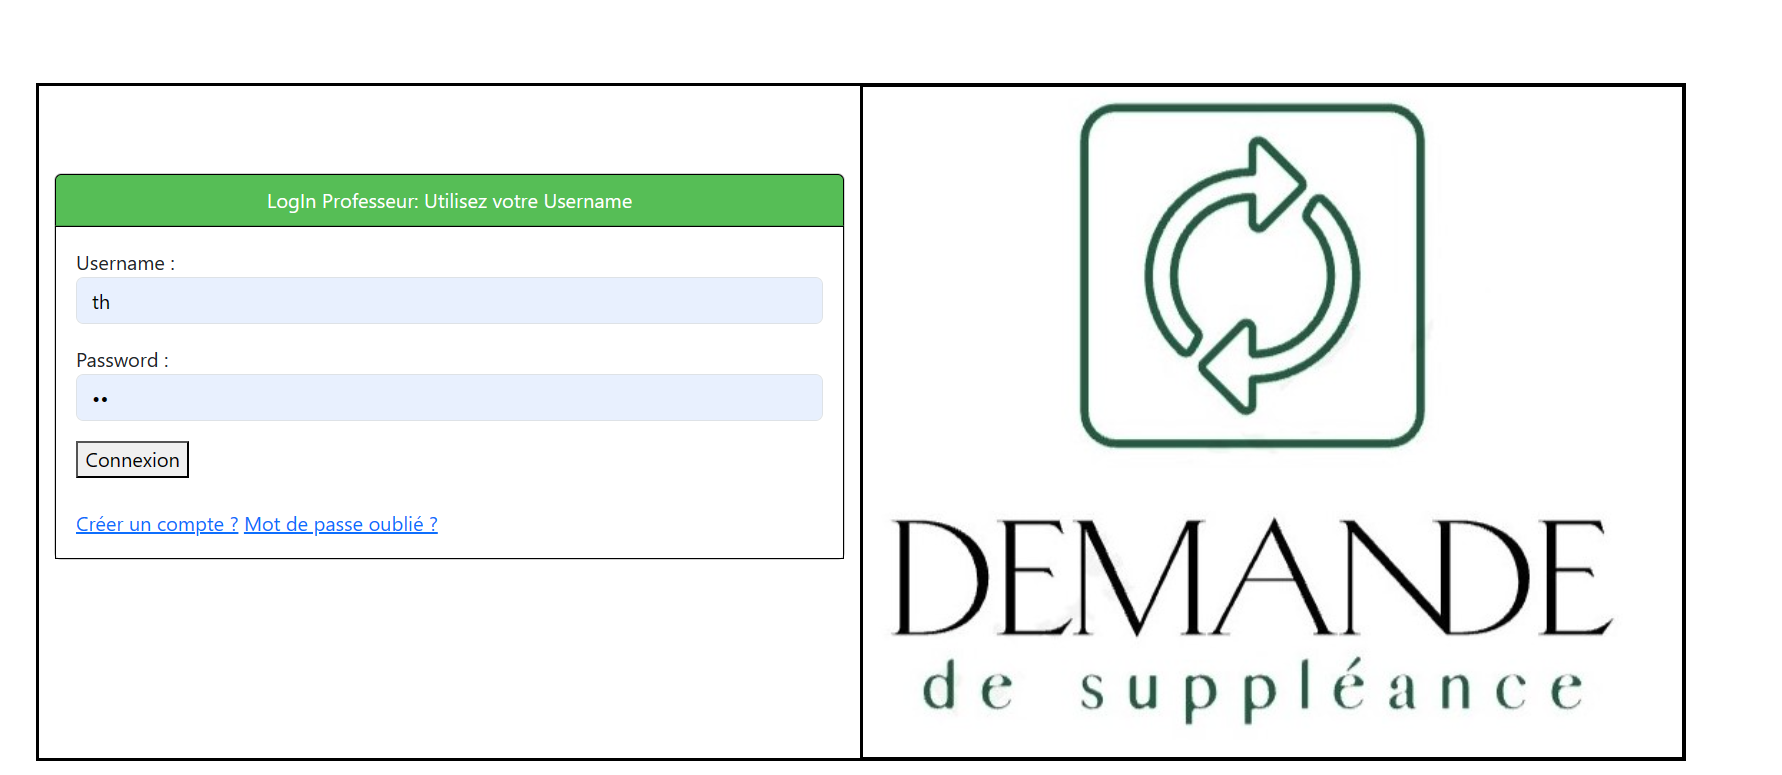
\includegraphics[width=0.7\textwidth]{loginprof.png}
\label{fig:im2} 
    \caption{Login Professor}
\end{figure}

Once there, you have the option to log in, reset your password, or create an account.

\subsection{Login}
To log in, you need your username and a password. Normally, you should have received a username and a temporary password if you were in the university's database at the launch of the app. If this is not the case, you can either contact the university or create an account by clicking on "créer un compte?" on figure 2 in section  \textcolor{blue}{\ref{fig:im2}}. For more details on how to create an account, refer to the section \textcolor{blue}{\ref{cree}}.
\subsection{Reset your passord / password forgot}
In the event that you have forgotten your password, simply click on the 'Mot de passe oublié?' link, as shown in figure 2 section \textcolor{blue}{\ref{fig:im2}}. This action will redirect you to the page shown in the figure below

\begin{figure}[H]
    \centering
 \fbox{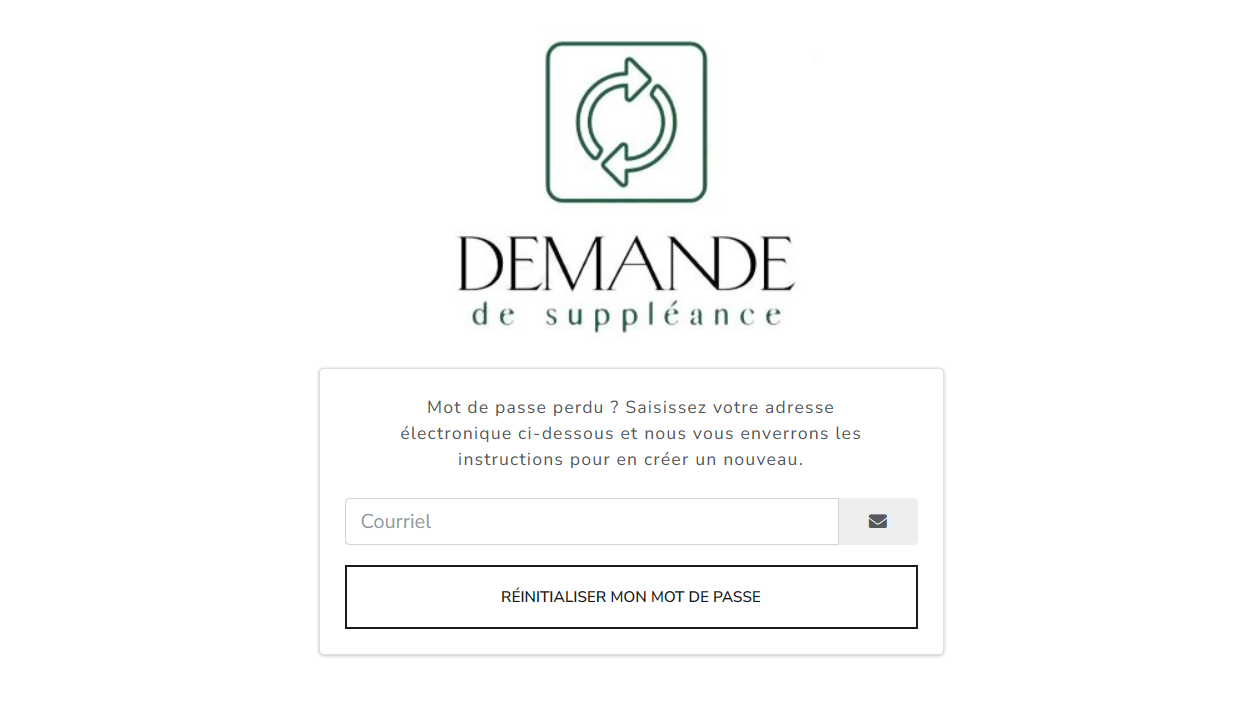
\includegraphics[width=0.7\textwidth]{motdepasse.png}}

    \caption{Password reset}
\end{figure}

When you reach the page, simply enter your Outlook address into the blank field labeled 'Courriel.' Afterward, you will receive an email containing a reset link, as demonstrated in figure 4 below. 
\begin{figure}[H]
    \centering
 \fbox{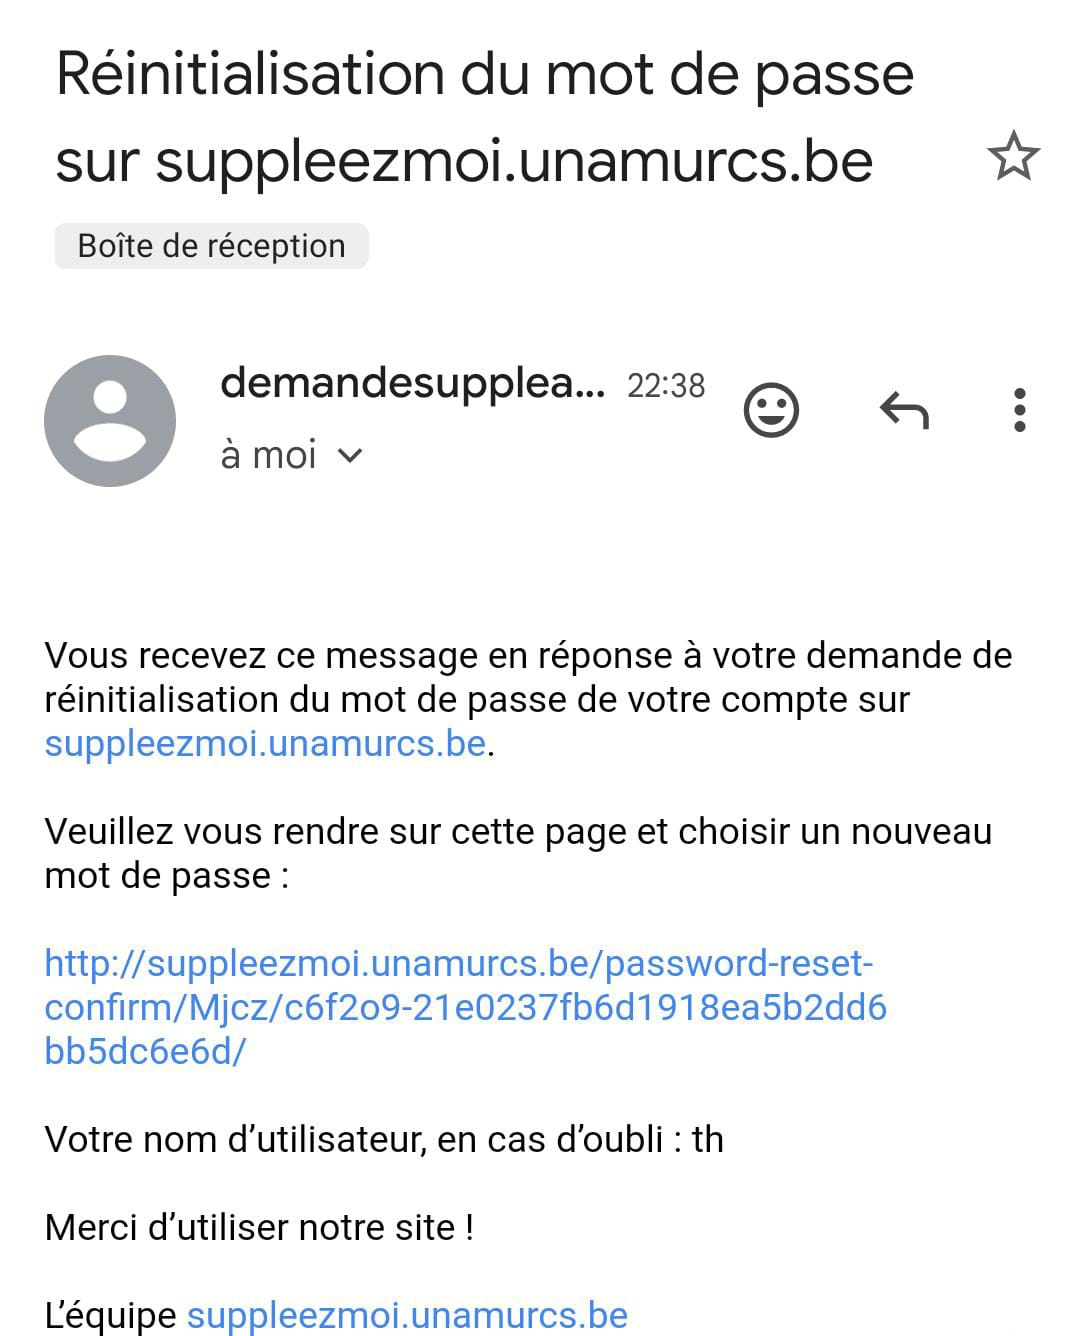
\includegraphics[width=0.5\textwidth]{Renitialise.jpg}}

    \caption{Password reset}
\end{figure}


Clicking on this link will lead you to the page illustrated in Figure 5. From there, you can proceed to reset your password by following the instructions and clicking on 'modifier mon mot de passe'. 



\begin{figure}[H]
    \centering
 \fbox{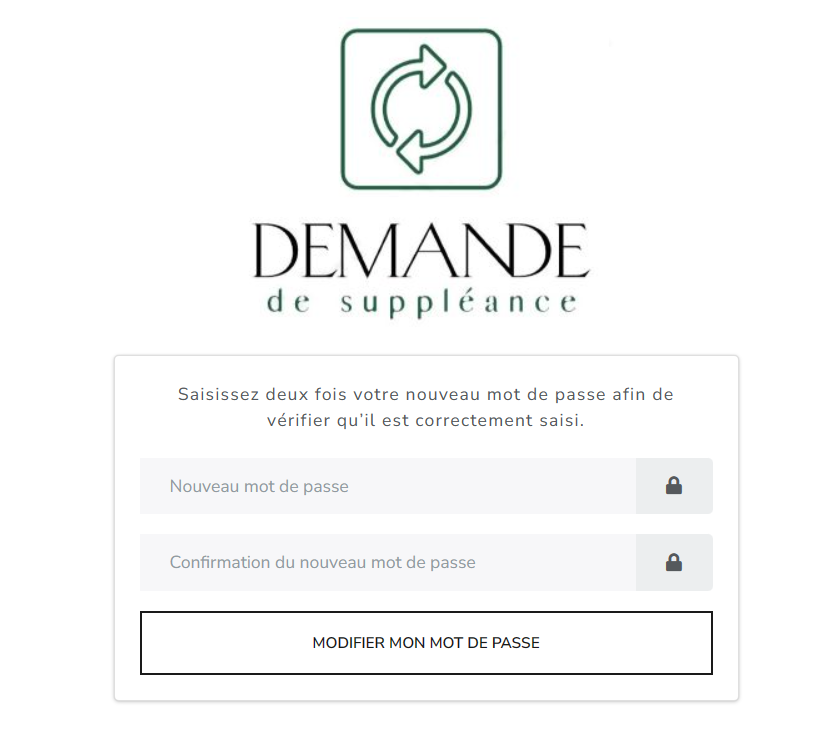
\includegraphics[width=0.5\textwidth]{renitial.png}}

    \caption{Password reset}
\end{figure}


\newpage
\subsection{Create an account}`\label{cree}

To create an account, simply click on the question "créer un compte?" as indicated in figure 2 section \textcolor{blue}{\ref{fig:im2}}. This action will prompt the appearance of the following page:

\begin{figure}[H]
    \centering
    \fbox{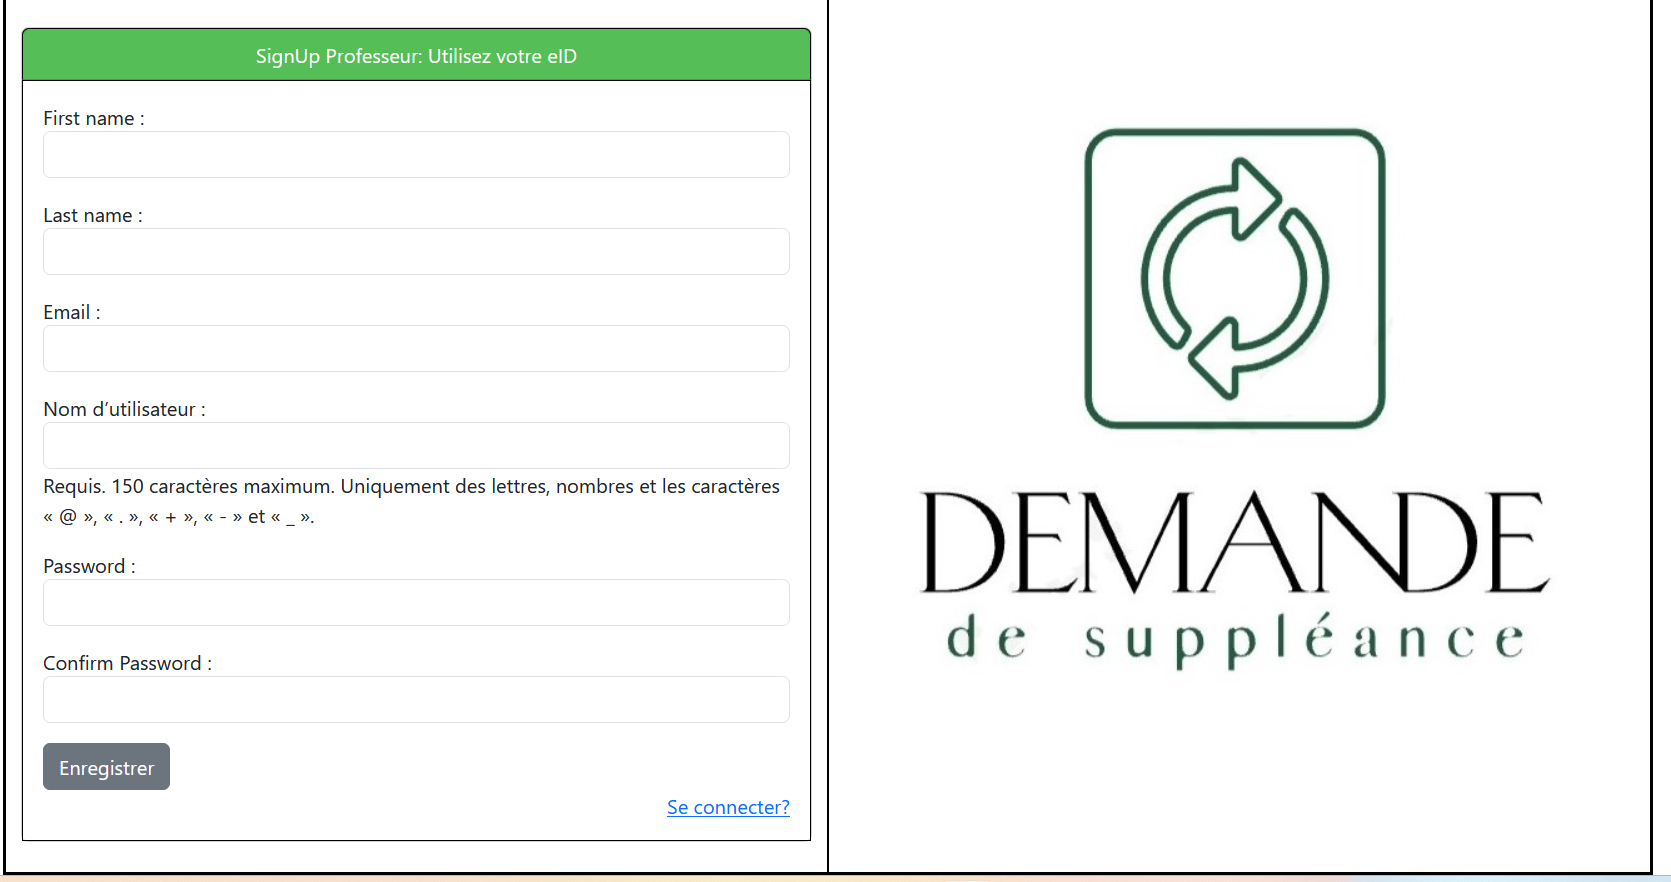
\includegraphics[width=0.7\textwidth]{image.png}}
    \caption{Create an account}
\end{figure}

Next, proceed to fill in your information. For the username, you can utilize your eid. If you don't have one, feel free to choose any desired username. Once done, save your information, and you will be automatically redirected to the login page.

\subsection{Navigating the Home Page for Professors}

After logging in, you will be directed to the home page for professors, as depicted in figure 7. On smaller screens, such as phones, the menu will appear differently, as shown in Figure 8, with a highlighted green row. Clicking on this row will expand the menu to display all available options, similar to  what is visible in figure 7.
\begin{figure}[H]
    \centering
    \fbox{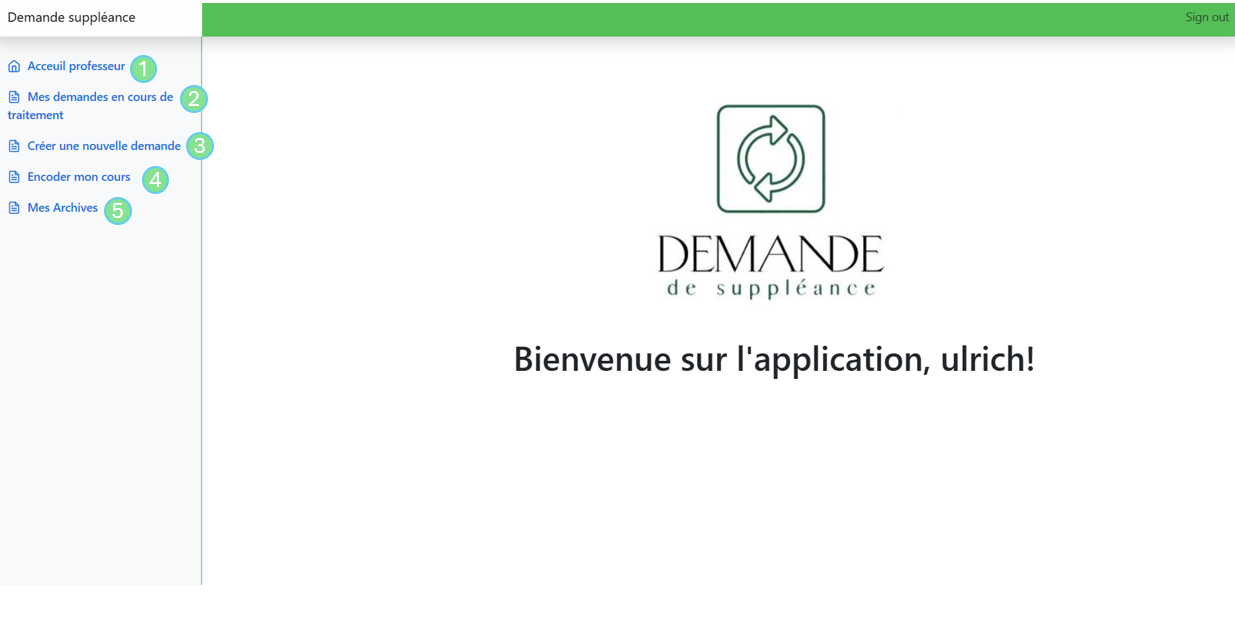
\includegraphics[width=0.7\linewidth]{image3.png}}
    \caption{Home page for professor}
    \label{7}
\end{figure}
\begin{figure}[H]
    \centering
    \fbox{
\includegraphics[width=0.5\linewidth]{image8.png}}
    \label{8}
    \caption{Home Page Mini screen}
\end{figure}

\subsubsection{Menu Options}\label{3}
\begin{description}
    \item[ 
"Accueil Professeur":] This option returns you to the home page for professors.

\item["Mes Demandes de Cours en Traitement":] Use this button to view all requests you have submitted that are awaiting processing by the administration. Refer to figure 9 for the layout of the redirected page.
\begin{figure}[H]
    \centering
    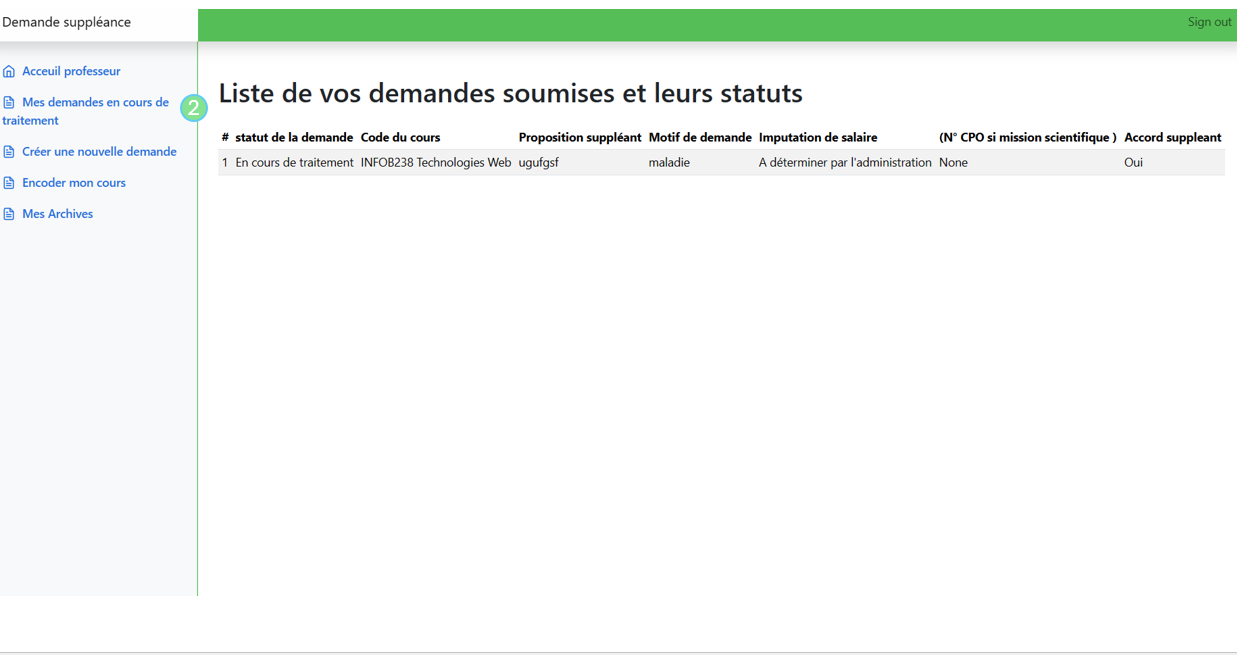
\includegraphics[width=0.75\linewidth]{image6.png}
    \caption{List Request}
\end{figure}

\item["Créer une Nouvelle Demande":]Clicking here allows you to initiate a new request, redirecting you to a form where you can input the necessary information (see figure 10).
\begin{figure}[H]
    \centering
    \fbox{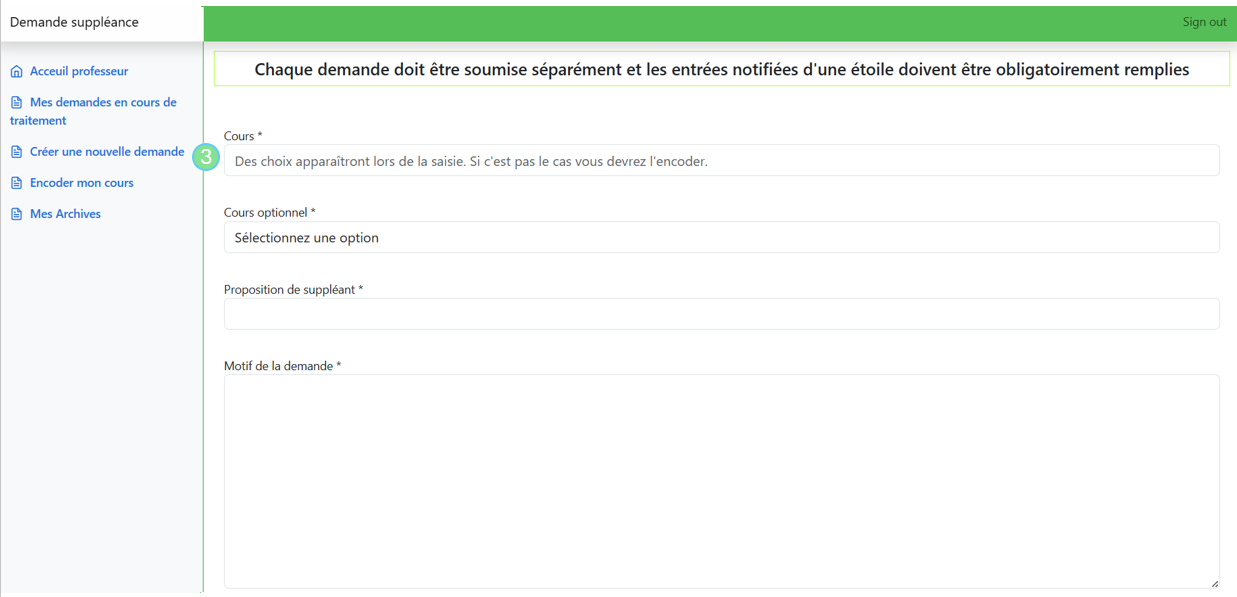
\includegraphics[width=0.75\linewidth]{image7.png}}
    \caption{form for request}
\end{figure}
\item["Encoder Mon Cours":] Select this option if your subject is not automatically listed when creating a new request. You'll need to manually input your subject details in the form provided  before proceeding with the request creation (see figure 11).
\begin{figure}[H]
    \centering
    \fbox{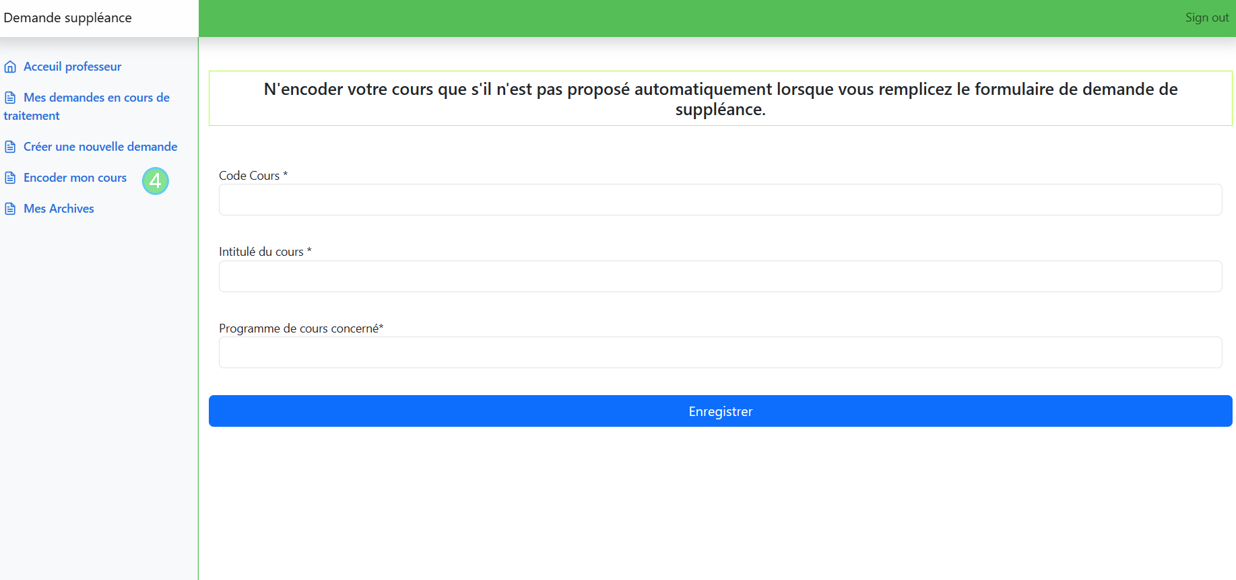
\includegraphics[width=0.75\linewidth]{image12.png}}
    \caption{Encode a course}
\end{figure}

\item["Archives Demandes":] Access all requests that have been processed by the university here. Requests may have statuses such as "Approuvé" (Approved), "Refusé" (Rejected), or "Était en Cours de Traitement" (Was Being Processed). If your request status is "Était en Cours de Traitement," it means your request was deleted by the administration before processing, and you should contact them for further asfistance (refer to Figure 12).
\begin{figure}[H]
    \centering
    \fbox{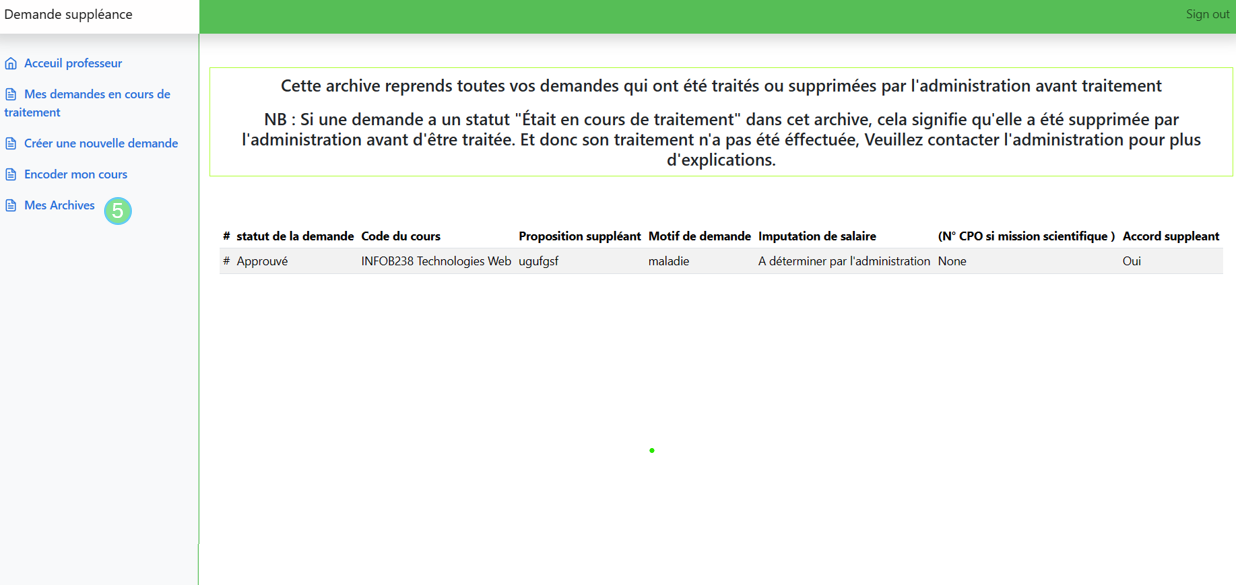
\includegraphics[width=0.75\linewidth]{image10.png}}
    \caption{Archive}
\end{figure}
\end{description}

\subsection{Creating a New Request}

To initiate a new request, follow the steps explained in  the previous sections to navigate to the home page for professors and click on "Créer une Nouvelle Demande." This action will display the form illustrated in figure 10 section \textcolor{blue}{\ref{3}}.

- For the "Cours" field, input the first letter or code of the course; a list of suggestions will appear, as shown in figure 13.
\begin{figure}[H]
    \centering
    \fbox{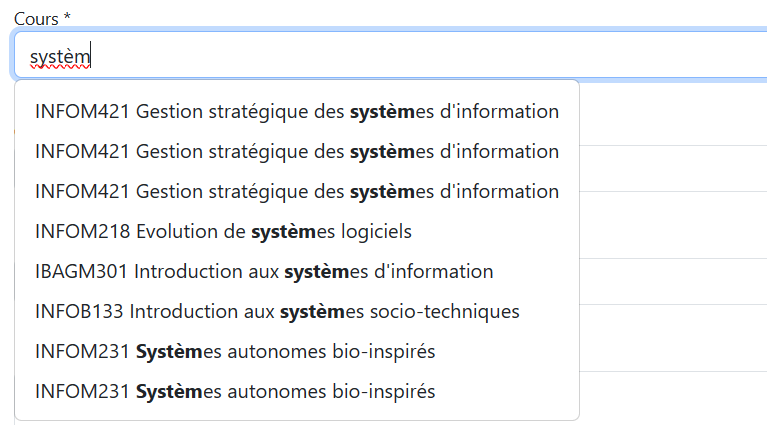
\includegraphics[width=0.75\linewidth]{image11.png}}
    \caption{Subjects}
\end{figure}
- In the "Cours Optionnel" field, choose between "Oui" (Yes) or "Non" (No) to indicate if the subject is optional (see Figure 14).
\begin{figure}[H]
    \centering
    \fbox{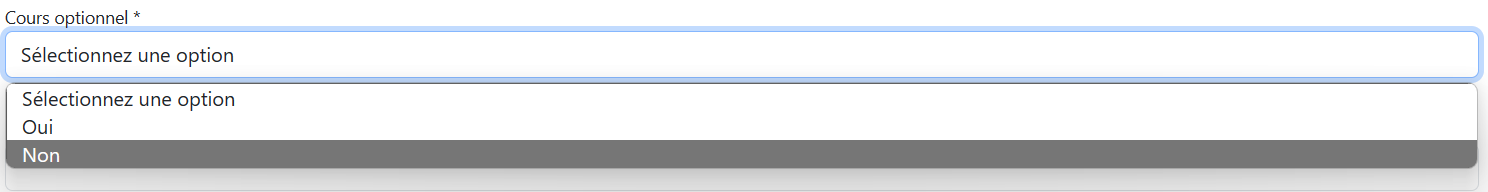
\includegraphics[width=0.75\linewidth]{image14.png}}
    \caption{option}
\end{figure}
- If you choose "Oui" (Yes), an alert will prompt, informing you that the course will only proceed if at least one person selects it (refer to Figure 15). Click "OK" to proceed.
\begin{figure}[H]
    \centering
    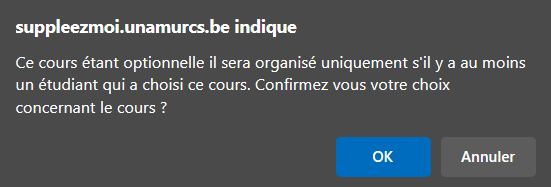
\includegraphics[width=0.75\linewidth]{image15.png}
    \caption{Alert}
\end{figure}

- Enter a substitute's name in the "Proposition de Suppléant" field and provide a reason for the request in the "Motif de la Demande" field.

- Select an option for "Imputation de Salaire" (see Figure 16). If you choose "Mission Scientifique," you'll need to fill in the "N°CPO" field (Figure 17); otherwise, it will be hidden.
\begin{figure}[H]
    \centering
    \fbox{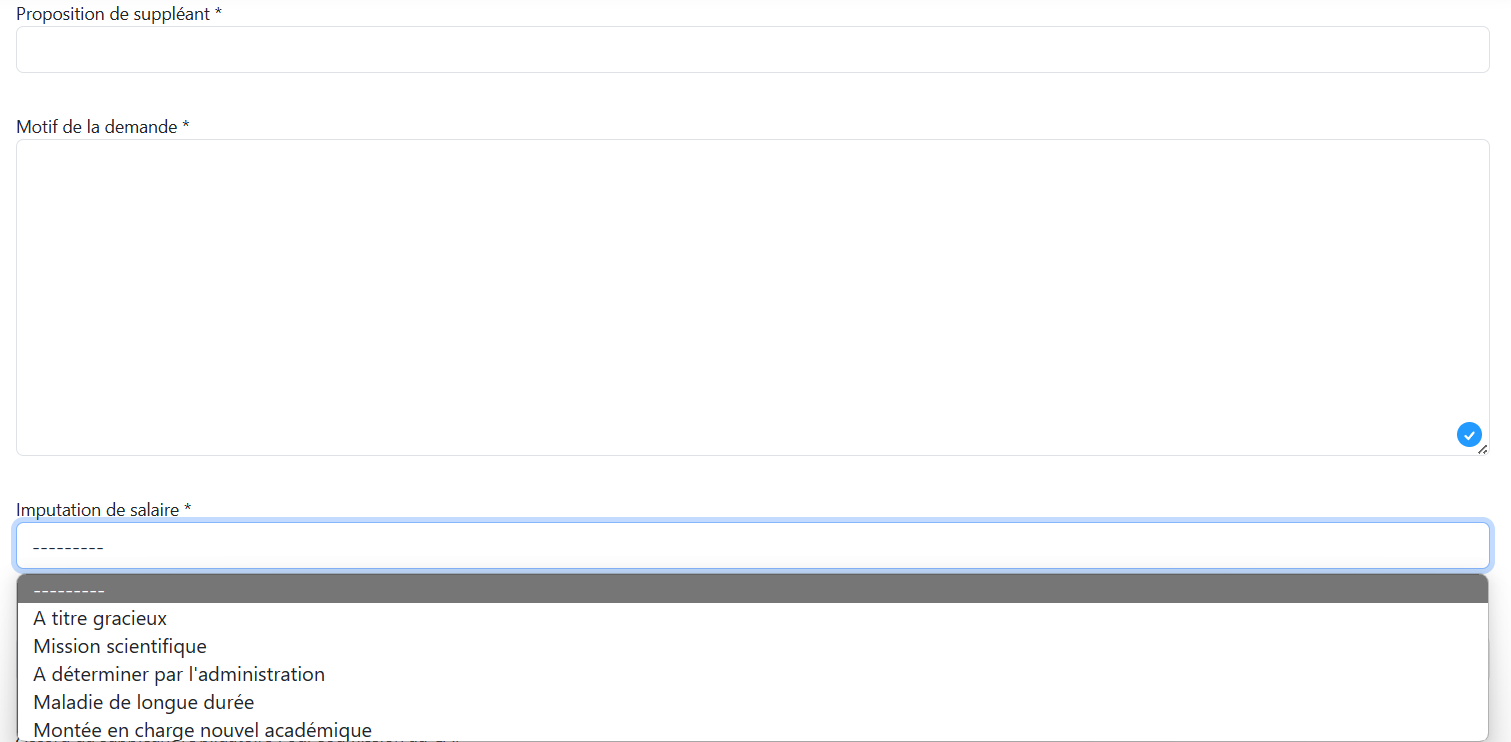
\includegraphics[width=0.75\linewidth]{image16.png}}
    \caption{form}
\end{figure}


- Indicate if the substitute is willing to substitute by selecting "Oui" (Yes), triggering a pop-up prompting you to send an email of agreement to the administration (see Figures 17 and 18).
\begin{figure}[H]
    \centering
    \fbox{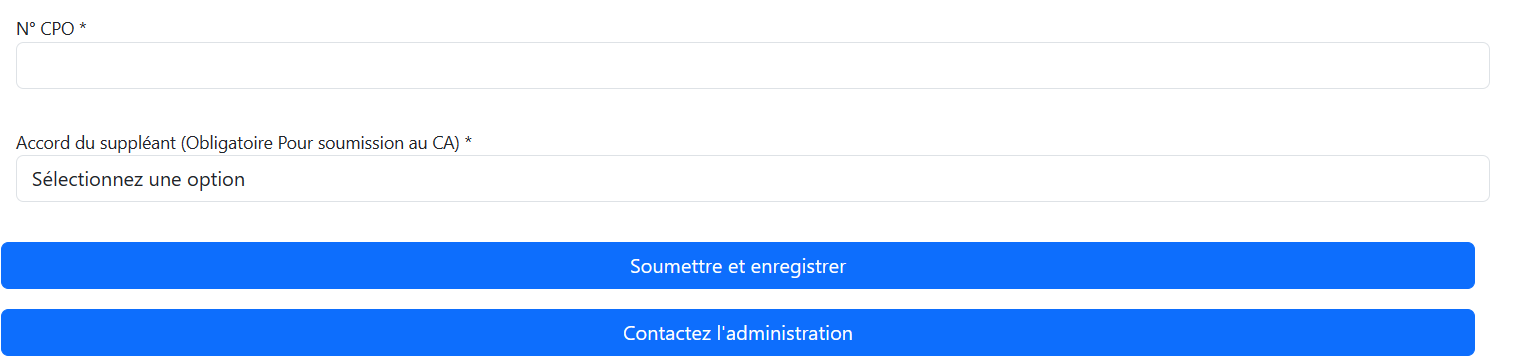
\includegraphics[width=0.75\linewidth]{image17.png}}
    \caption{rest of the form}
\end{figure}

\begin{figure}[H]
    \centering
    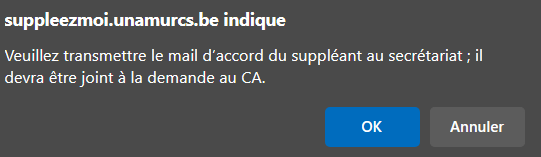
\includegraphics[width=0.75\linewidth]{image18.png}
    \caption{Pop-up for the email}
\end{figure}
- Once all fields are filled, click on "Soumettre et Enregistrer" to submit the request. To contact the administration, click on "Contacter l'Administration," as shown in Figure 17.

\section{Using the Application as an Administrator}

When you click on the "Administrateur" button (figure 1 section \textcolor{blue}{\ref{fig:im1}}), you will be redirected to the administrator login page, as depicted below:

\begin{figure}[H]
    \centering
    \fbox{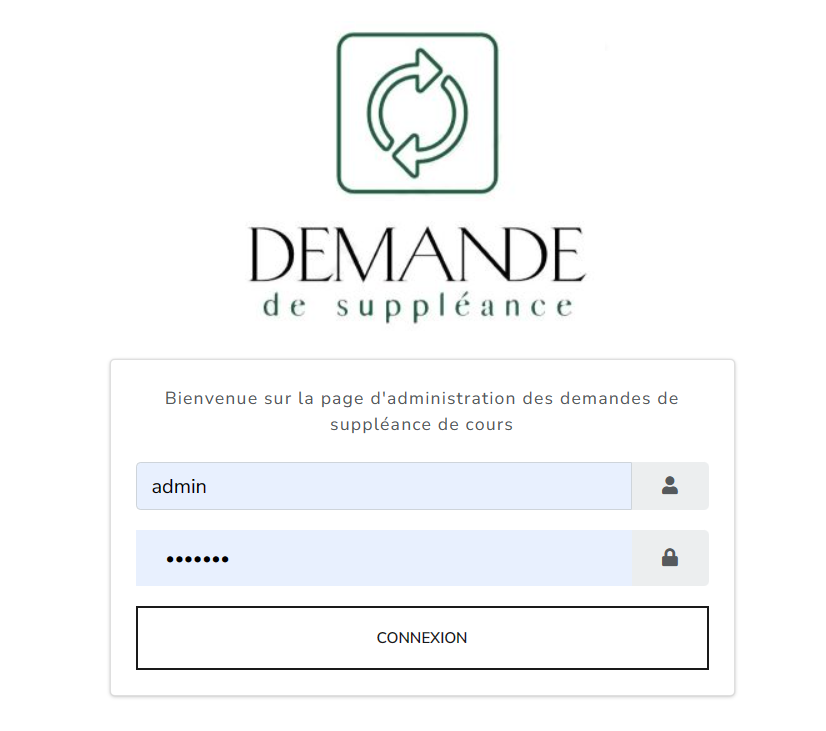
\includegraphics[width=0.75\linewidth]{image19.png}}
    \caption{Administrator Login Page}
\end{figure}

To access the admin area, fill in the login credentials and click on the "Connexion" button. Once logged in, you will be directed to the Admin Home Page, shown below:

\begin{figure}[H]
    \centering
    \fbox{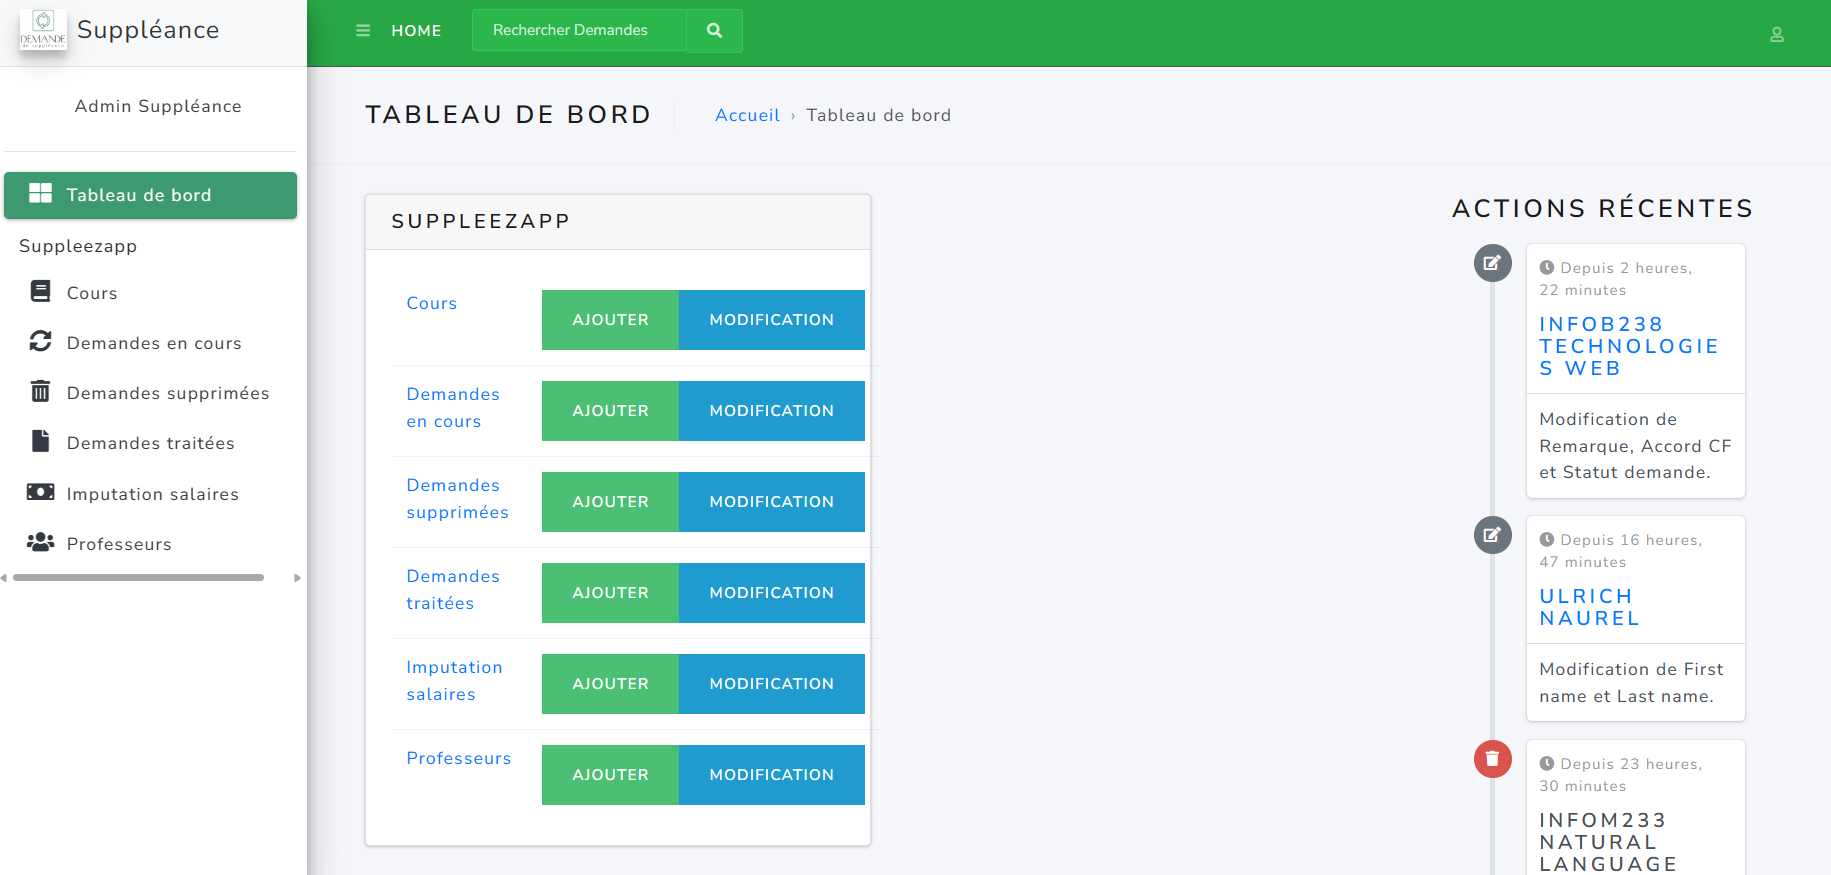
\includegraphics[width=0.75\linewidth]{image20.png}}
    \caption{Admin Home Page}
\end{figure}

\subsection{Recent Actions}

The "Actions Récentes" section displays a history of recent actions performed in the admin interface, including deletions, modifications, or insertions, along with a summary of each action:

\begin{figure}[H]
    \centering
    \fbox{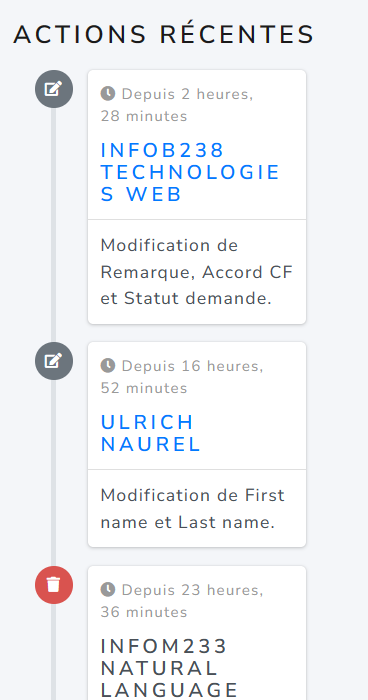
\includegraphics[width=0.3\linewidth]{image21.png}}
    \caption{Recent Actions}
\end{figure}

\subsection{SUPPLEEZAPP Section}

Under the "SUPPLEEZAPP" section (Figure 22), you'll find a summary of all available tables within the app. You can quickly add a new entry to any table by clicking on the "Ajouter" button next to the table name. Similarly, you can edit an existing entry by selecting "Modification."

\begin{figure}[H]
    \centering
    \fbox{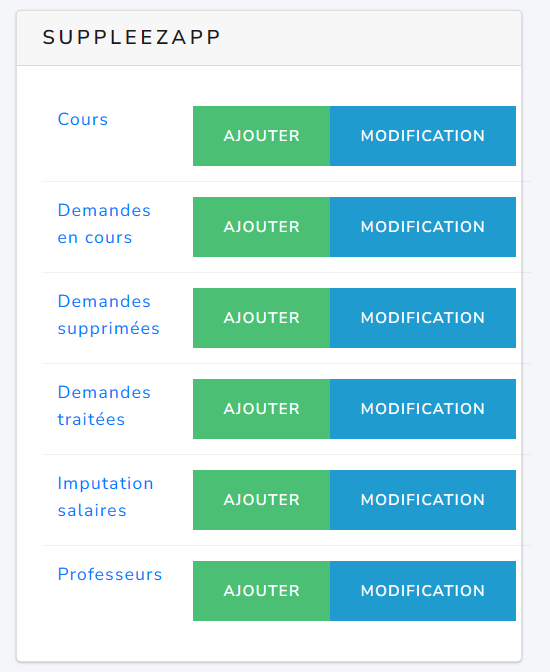
\includegraphics[width=0.3\linewidth]{image22.png}}
    \caption{SUPPLEEZAPP Overview}
\end{figure}

\subsection{Side Bar Menu}

The side bar menu enables navigation to different sections and pages of the app. Clicking on "Tableau de Bord" will redirect you to the home page:

\begin{figure}[H]
    \centering
    \fbox{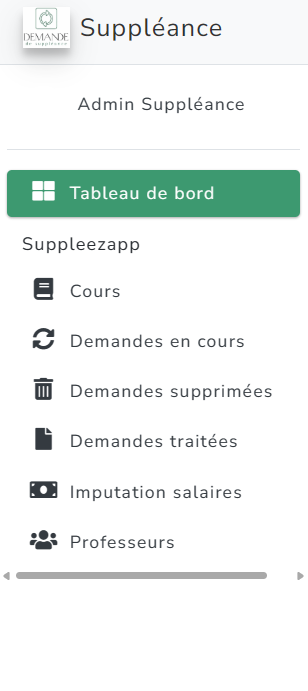
\includegraphics[width=0.3\linewidth]{image23.png}}
    \caption{Side Bar Menu}
\end{figure}

\subsection{Managing Courses}

Clicking on "Cours" redirects you to the page shown below:

\begin{figure}[H]
    \centering
    \fbox{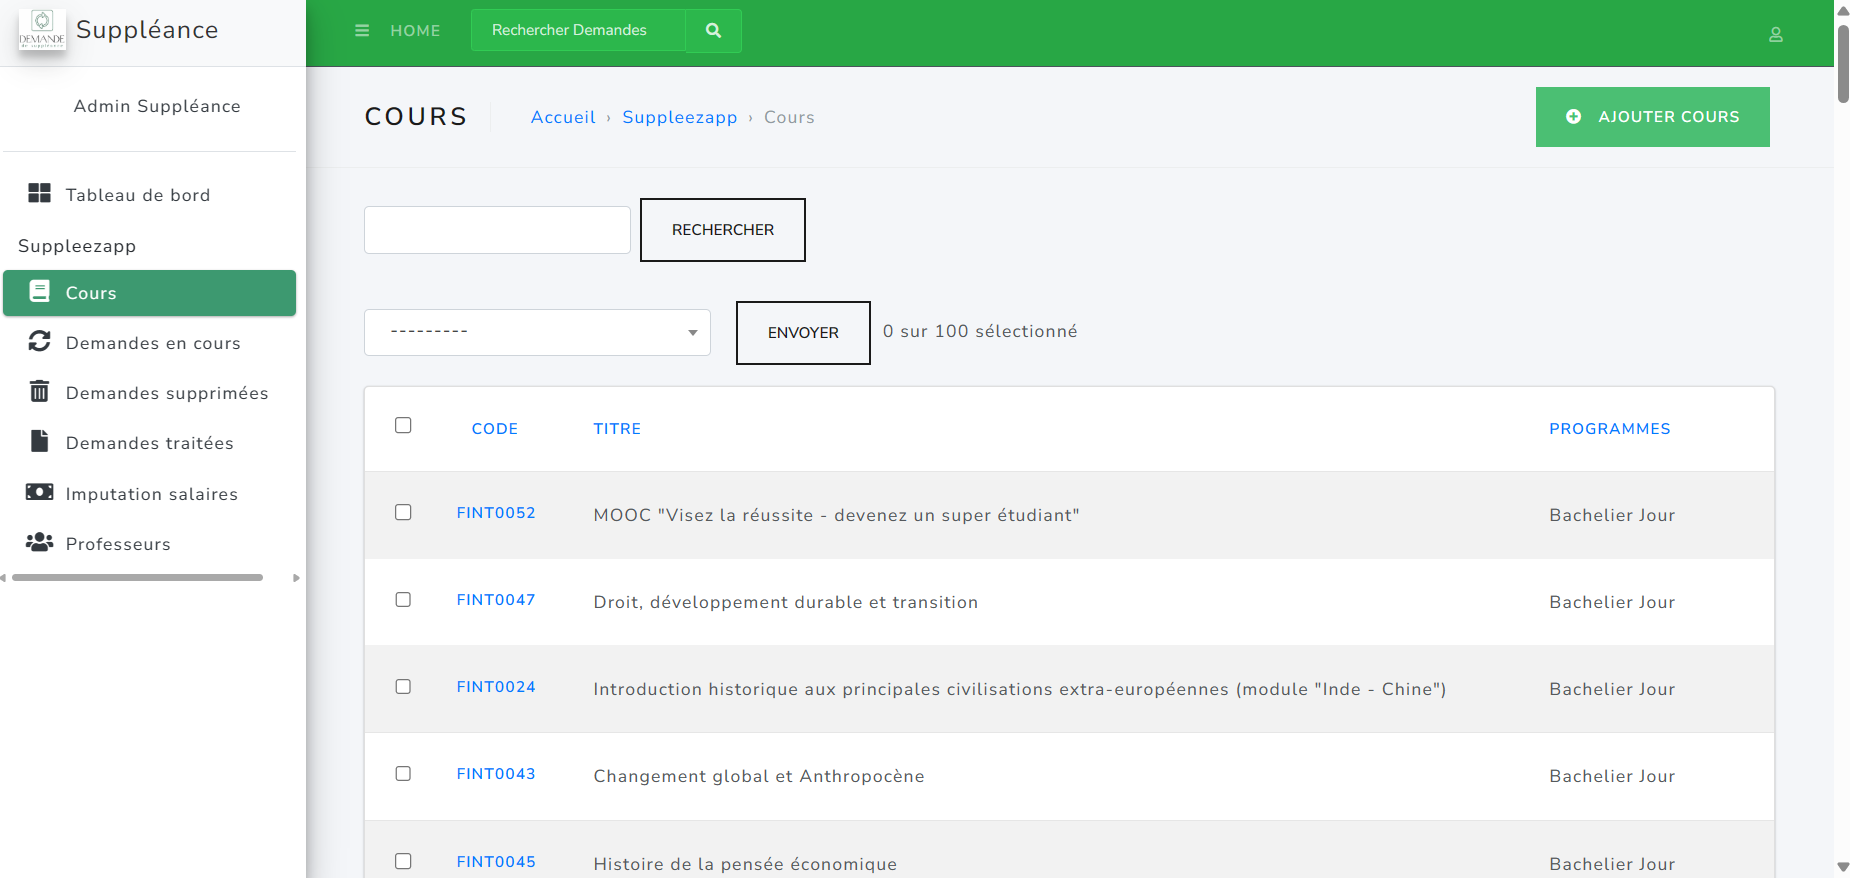
\includegraphics[width=0.75\linewidth]{image24.png}}
    \caption{Courses Page}
\end{figure}

Here, you can view a list of all available courses. You can even find a specific course by using the "rechercher" button after entering a keyword. To add a new course, click on "ajouter cours" at the top corner.For more details on adding a new course, refer to the section \textcolor{blue}{\ref{13}} on adding a course as administrator. To delete one or more selected courses, select "supprimer les cours sélectionnés" and then click on the "Envoyer" button:

\begin{figure}[H]
    \centering
    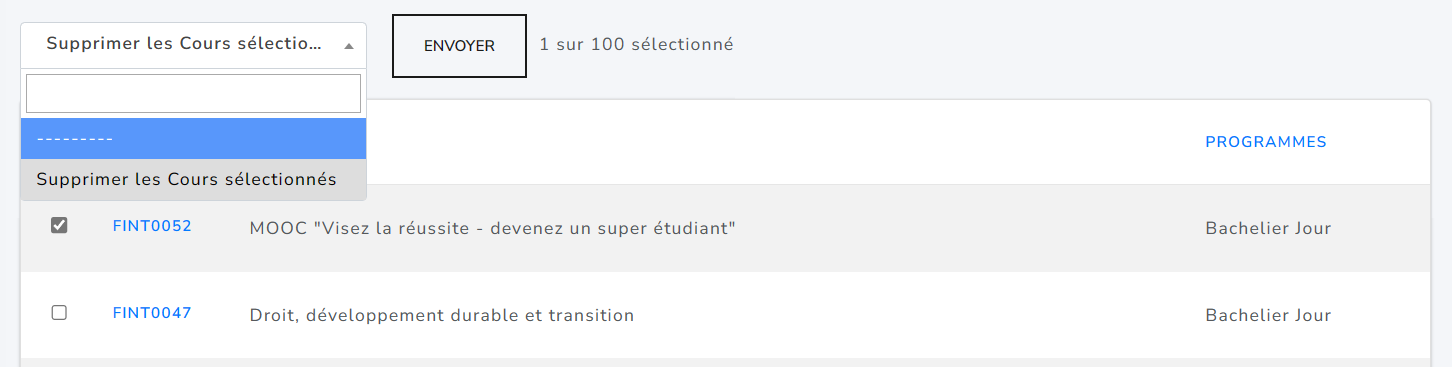
\includegraphics[width=0.75\linewidth]{image26.png}
    \caption{Deleting a Course}
\end{figure}

For confirmation, you will be prompted to either confirm or cancel the action. Confirm by clicking on "oui je suis sûr":

\begin{figure}[H]
    \centering
    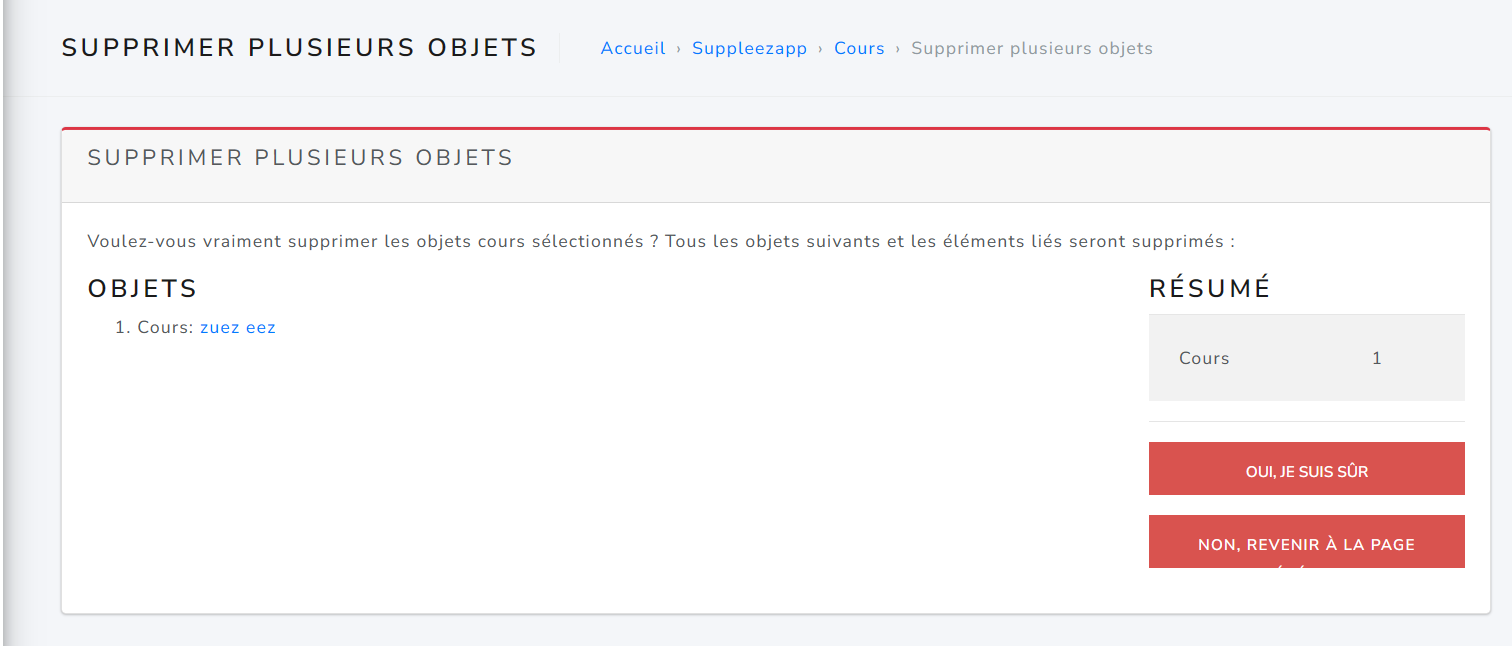
\includegraphics[width=0.75\linewidth]{image27.png}
    \caption{Confirmation for Deletion}
\end{figure}

\subsection{Managing Requests}

Selecting "Demandes en Cours" displays a list of requests submitted by professors:

\begin{figure}[H]
    \centering
    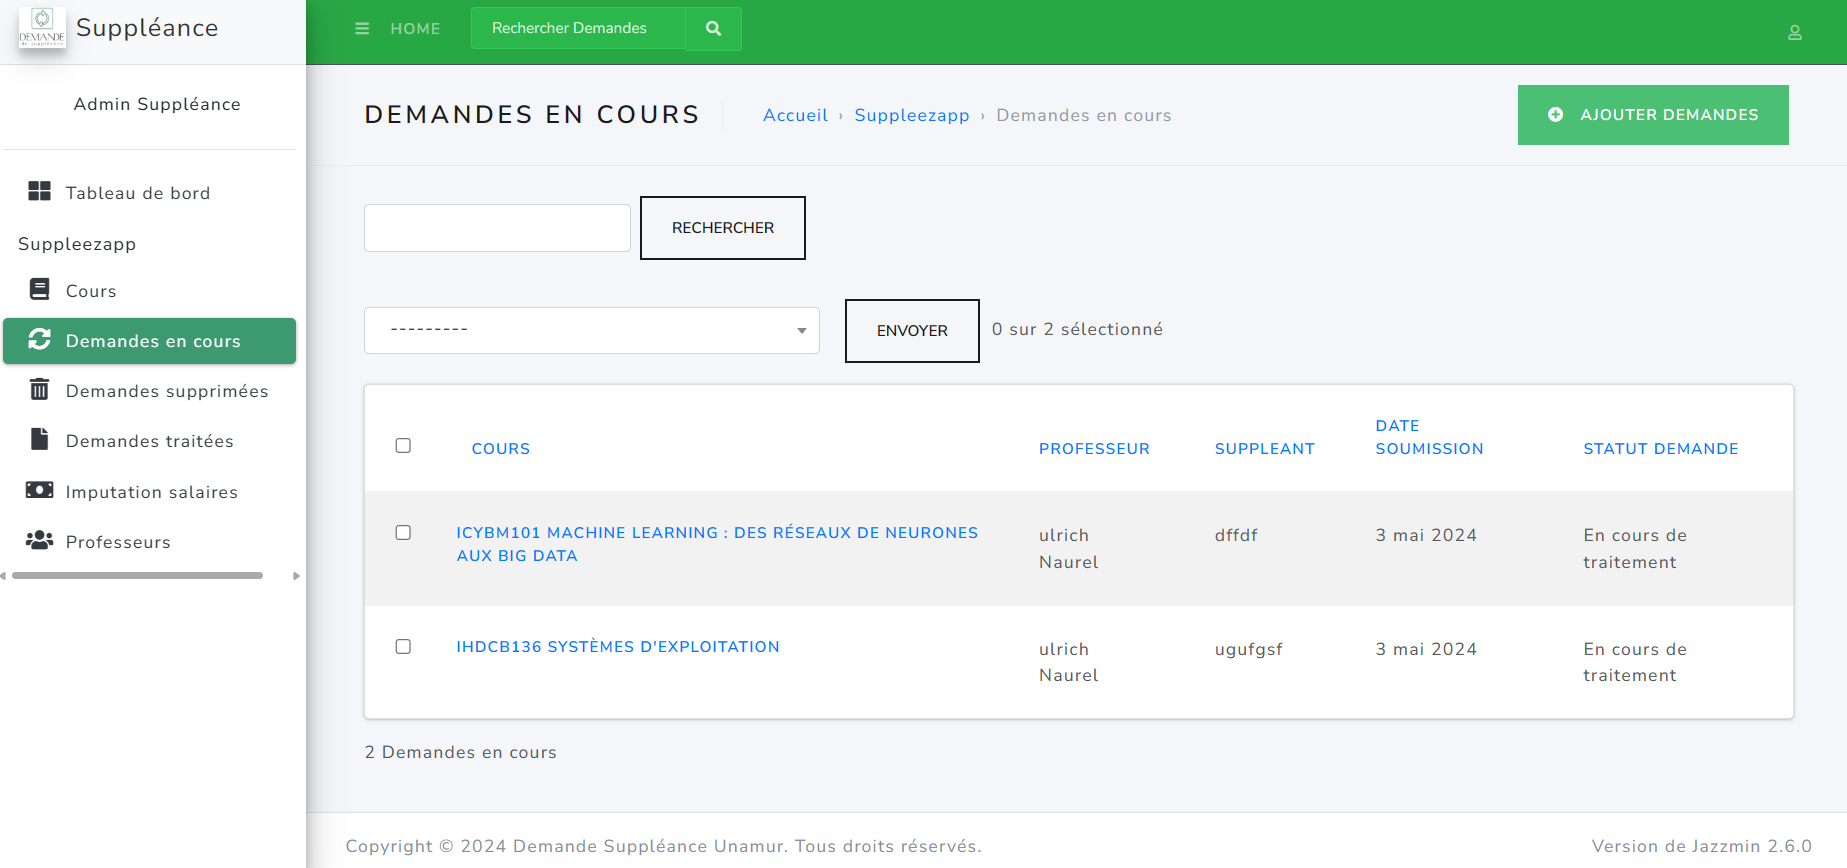
\includegraphics[width=0.75\linewidth]{image28.png}
    \caption{Requests}
\end{figure}

To add a new request, click on "Ajouter Demande" in the top right corner. For extra details on creating a new request, refer to the section\textcolor{blue}{\ref{12}} on creating requests in the admin session. You can also delete requests and download all submitted requests in an Excel file.You just have to first select your request, then select and action  between the deleting or downloading and then click on "Envoyer". illustration: 
\begin{figure}[H]
    \centering
    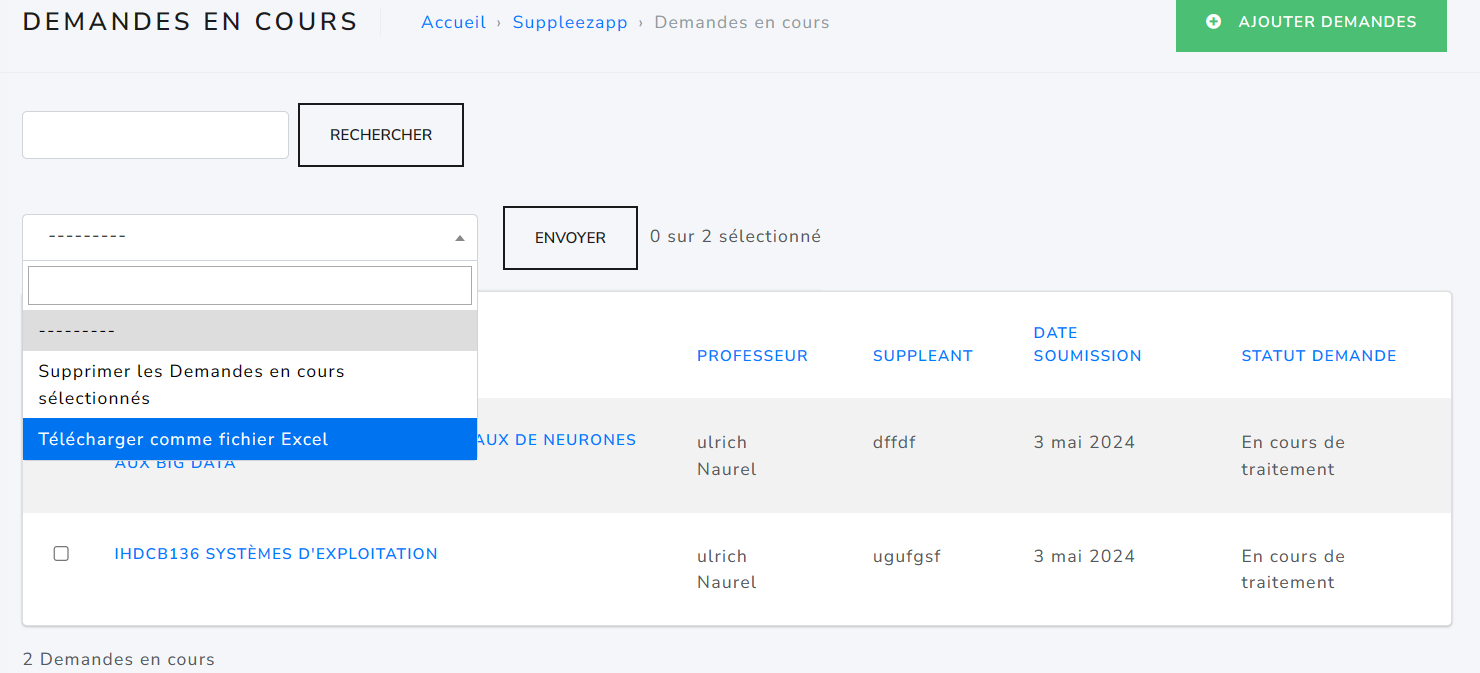
\includegraphics[width=0.75\linewidth]{image31.png}
    \caption{Delete or Download request as Excel File}
\end{figure}
When you click on "Demandes supprimées" you will see a list of all the requests that have been deleted. From there, you can choose to either delete them permanently or download them, as explained before.

Similarly, when you click on "Demandes traitées" you will find a list of requests that have already been handled. The process for using the button is the same as explained in the section for the "Demandes en cours" button.

\begin{figure}[H]
    \centering
    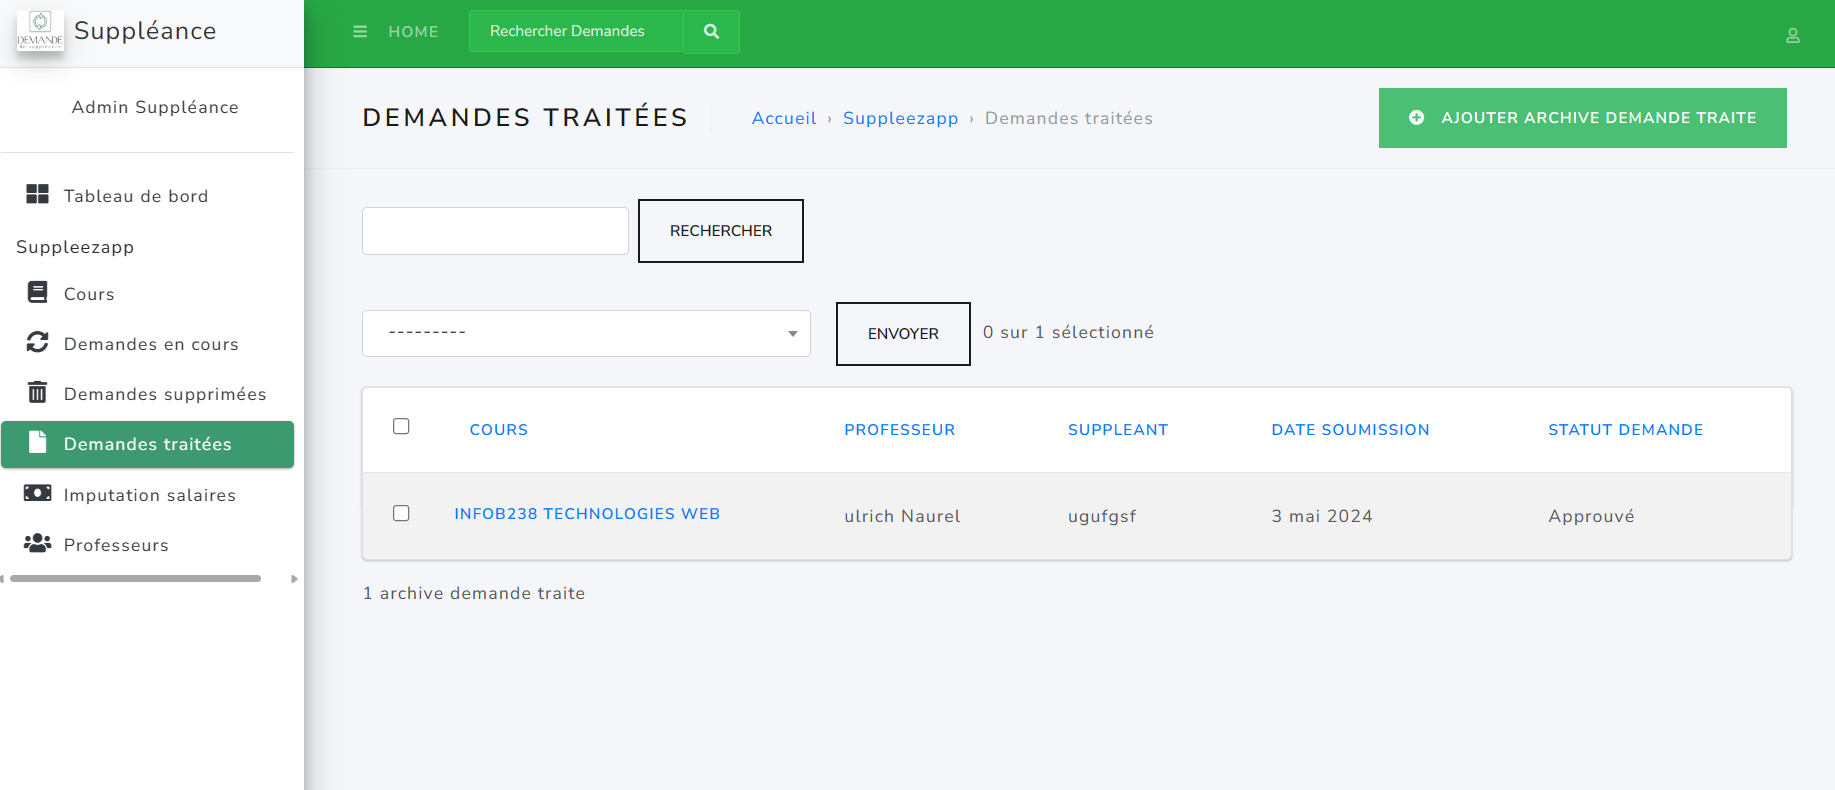
\includegraphics[width=0.75\linewidth]{image33.png}
    \caption{Processed Requests}
\end{figure}

When you click on "imputation de salaire" you have the table on the figue below.
\begin{figure}[H]
    \centering
    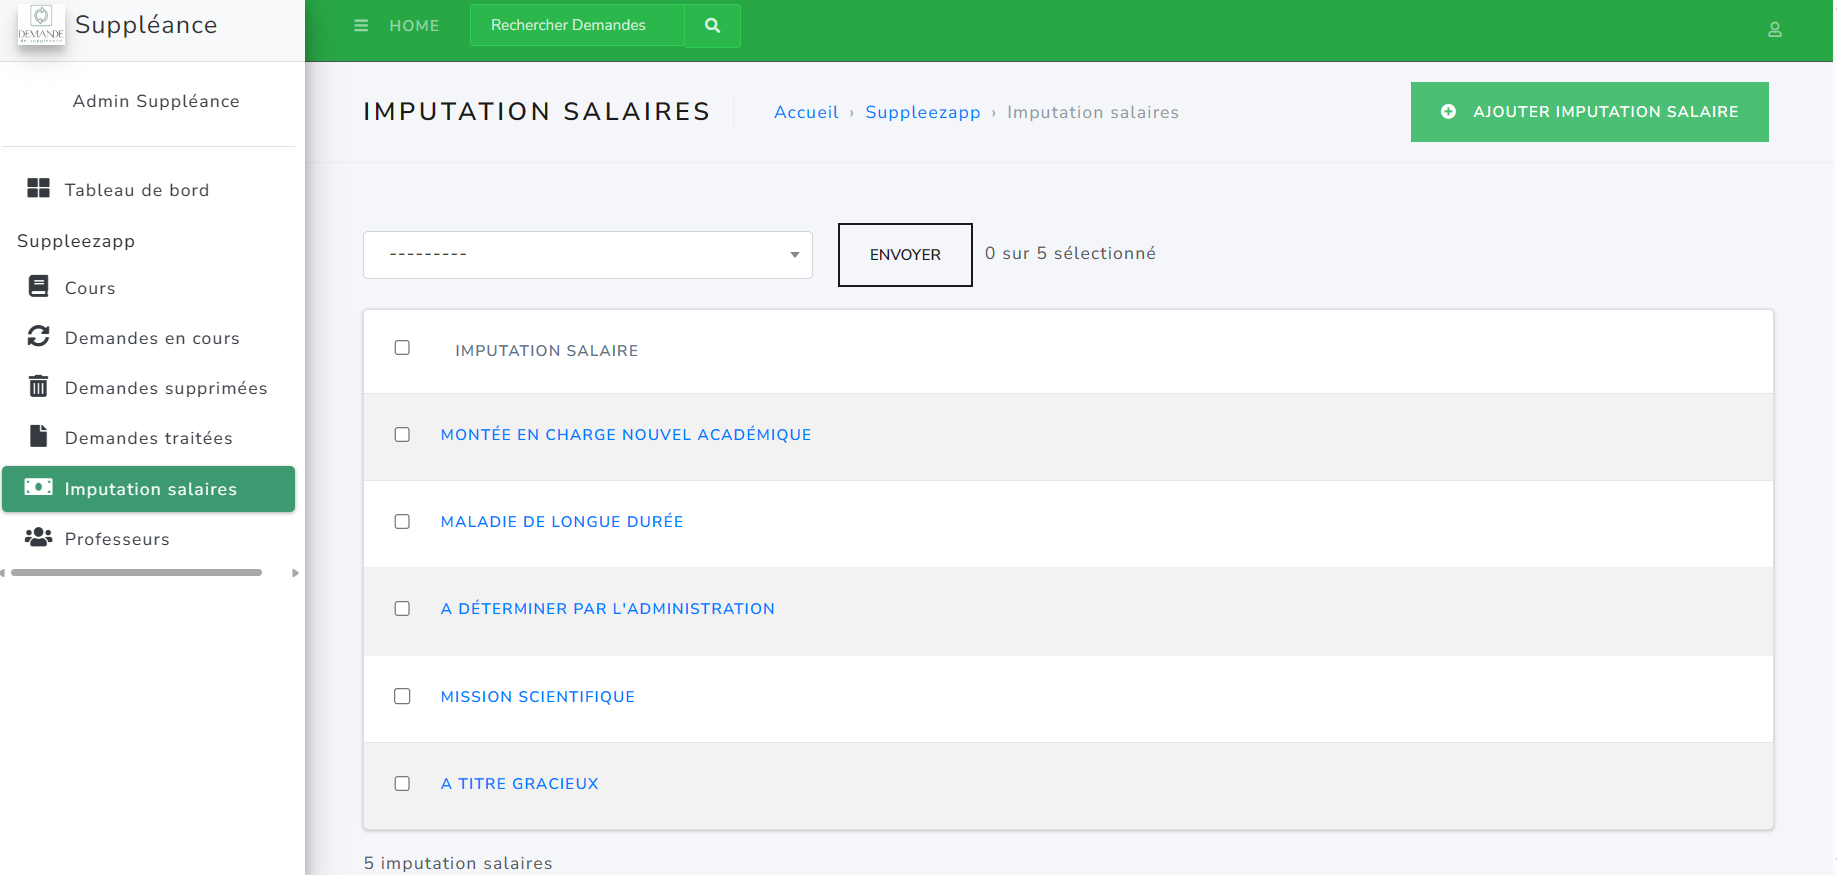
\includegraphics[width=0.75\linewidth]{image35.png}
    \caption{Enter Caption}
\end{figure}
Here you have the possibility to add more option for the imputation of salary by clicking on the corner at top at the rigth.
you will be redirected to the page below where you just have to enter the new imputation and then click on "enregistrer" to  save it. 
\begin{figure}[H]
    \centering
    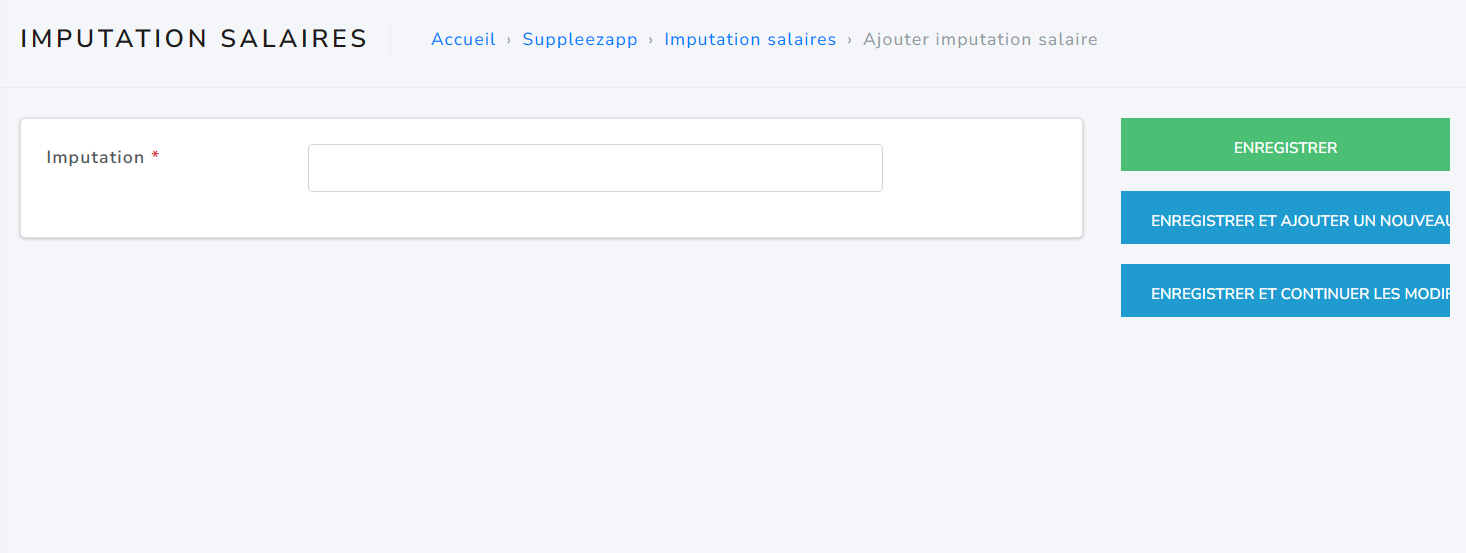
\includegraphics[width=0.75\linewidth]{image36.png}
    \caption{Enter Caption}
\end{figure}


\subsection{Managing Users}

Clicking on "Professeur" displays a list of all professors using the app. You can add a new professor by clicking on "Ajouter Professeur",for more details refer to the section \textcolor{blue}{\ref{11}}. To delete or search for a specific user, follow similar steps as for deleting or finding a course.

\begin{figure}[H]
    \centering
    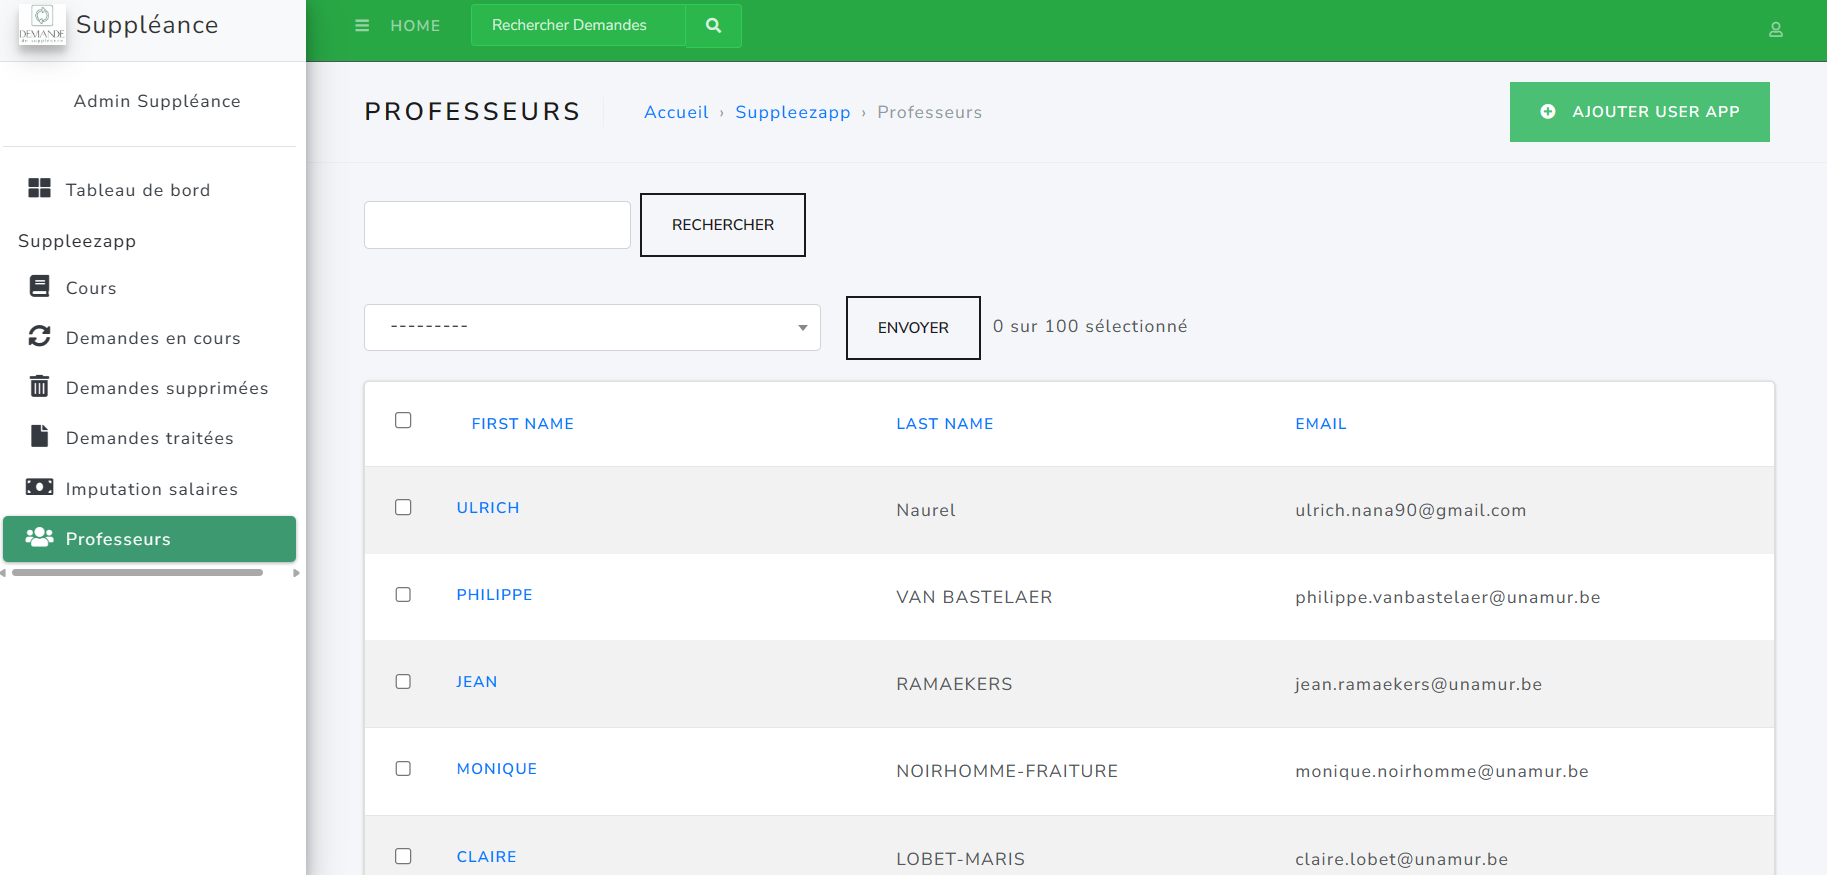
\includegraphics[width=0.75\linewidth]{image37.png}
    \caption{Managing Users}
\end{figure}

Additionally, you can select one or more users and send them an email containing their account information and a temporary password for initial login:

\begin{figure}[H]
    \centering
    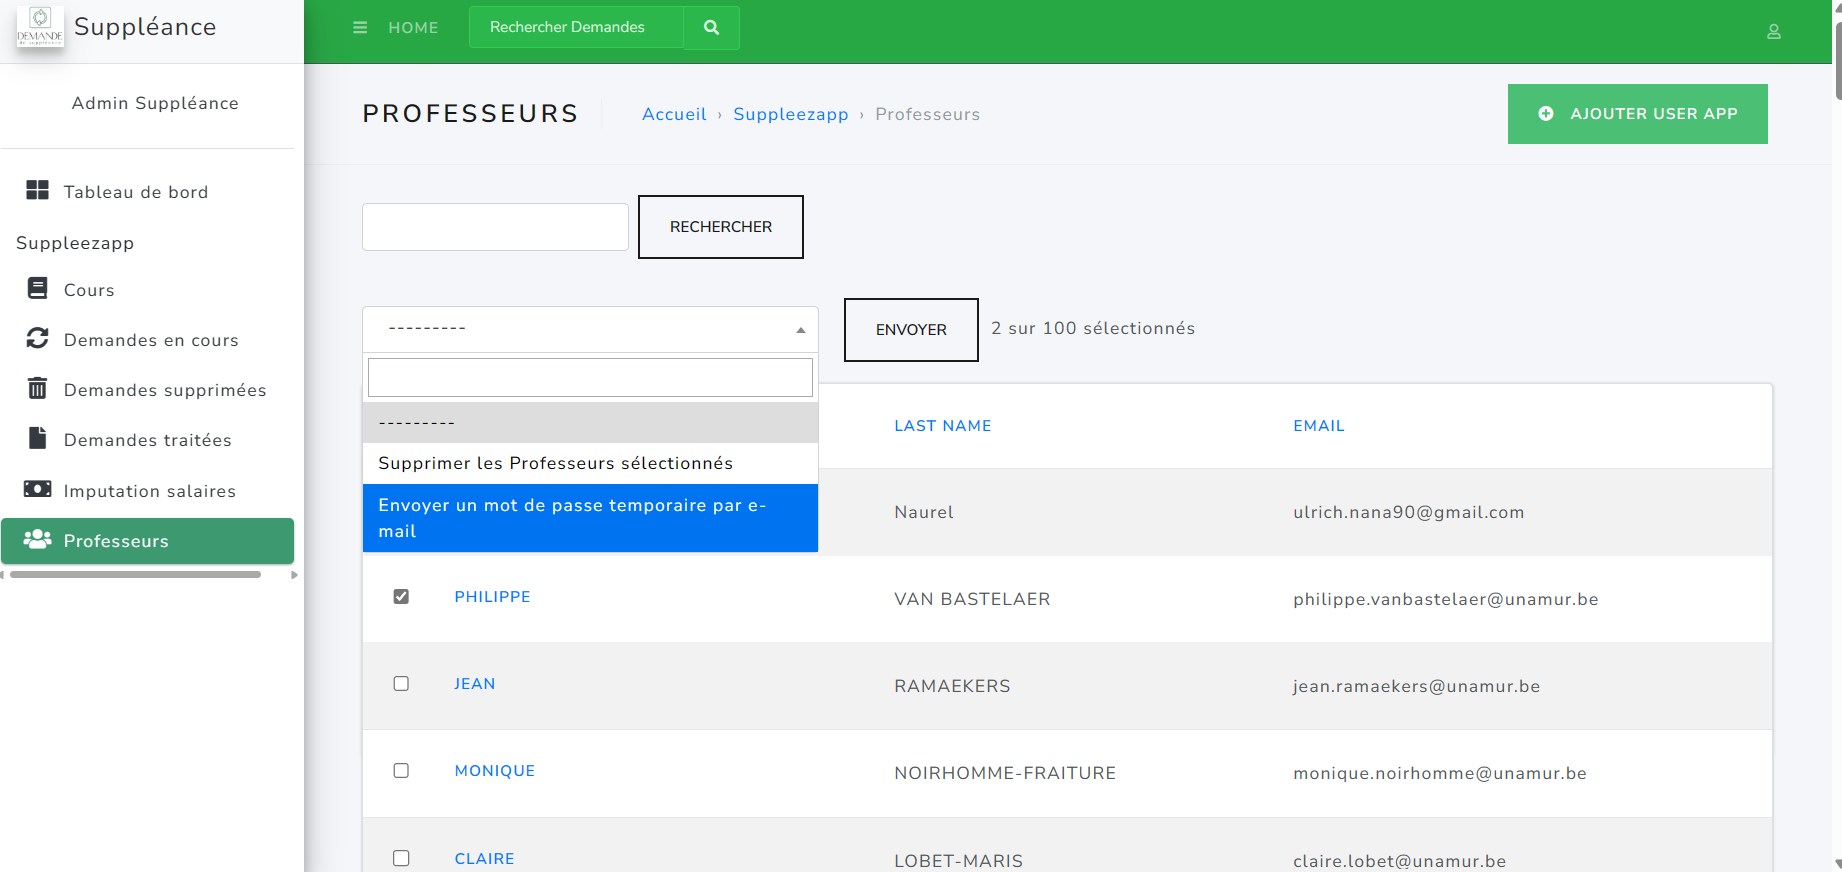
\includegraphics[width=0.75\linewidth]{image38.png}
    \caption{Sending Email to Users}
\end{figure}

For detailed instructions on adding a professor or creating a request, refer to the respective sections.
\subsection{Managing Data}

\subsubsection{Adding a Professor}  \label{11}

To add a professor, follow these steps:

\begin{enumerate}
    \item Begin by navigating to the section for adding professors.
    \item Fill in the necessary information for the professor, such as name, email, and any other required details.
    \item Once all information is entered, click on the "Enregistrer" button located at the top right corner of the page.
\end{enumerate}

\begin{figure}[H]
    \centering
    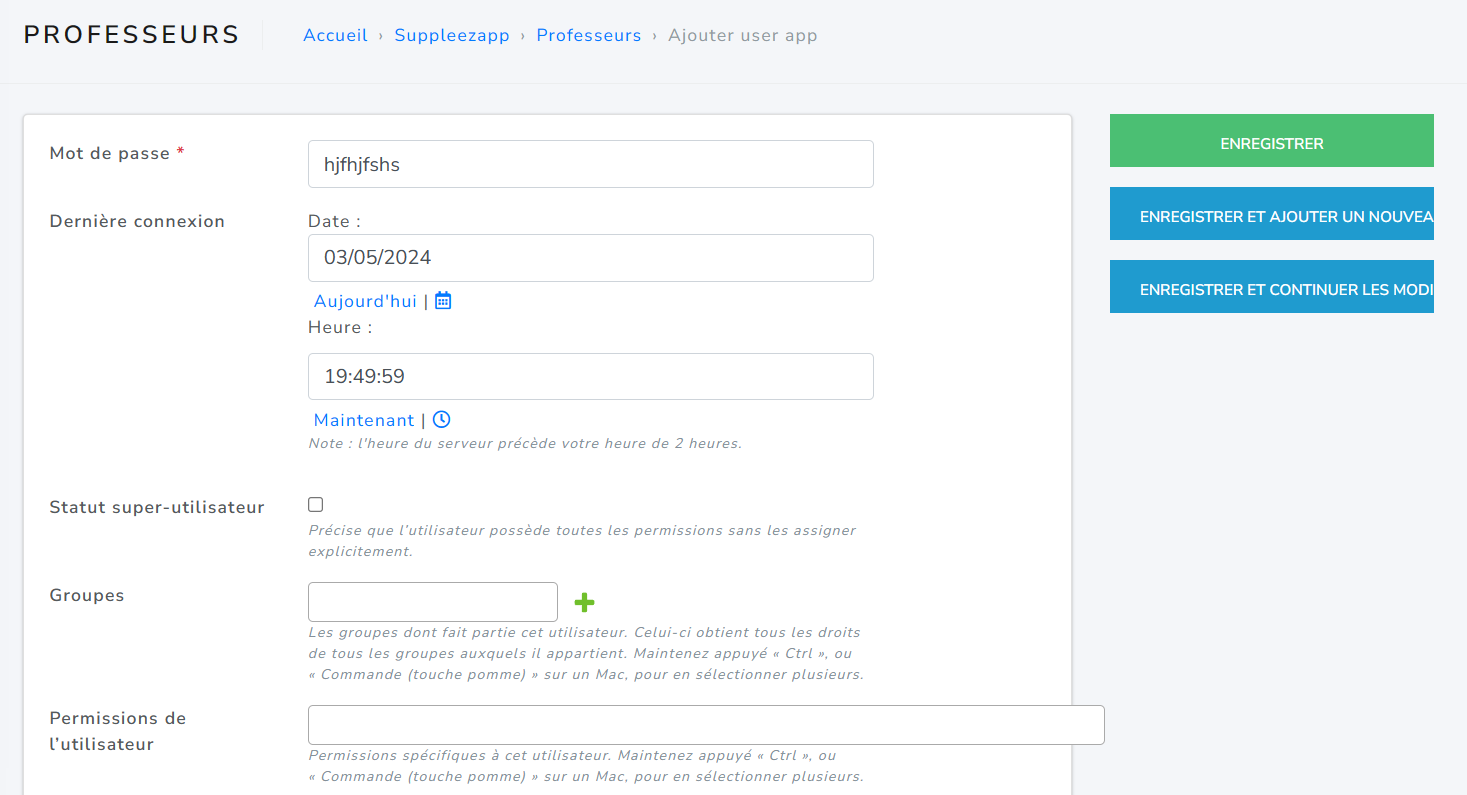
\includegraphics[width=0.75\linewidth]{image40.png}
    \caption{Adding a Professor - Step 1}
\end{figure}

\begin{figure}[H]
    \centering
    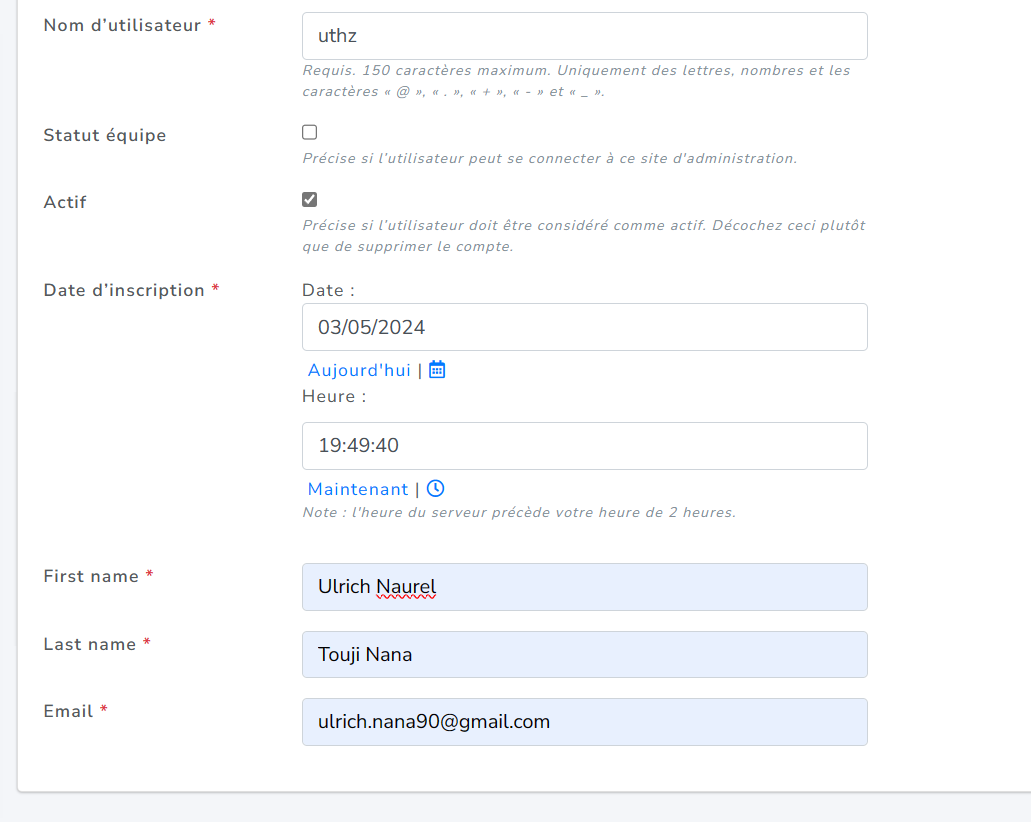
\includegraphics[width=0.75\linewidth]{image41.png}
    \caption{Adding a Professor - Step 2}
\end{figure}

\begin{figure}[H]
    \centering
    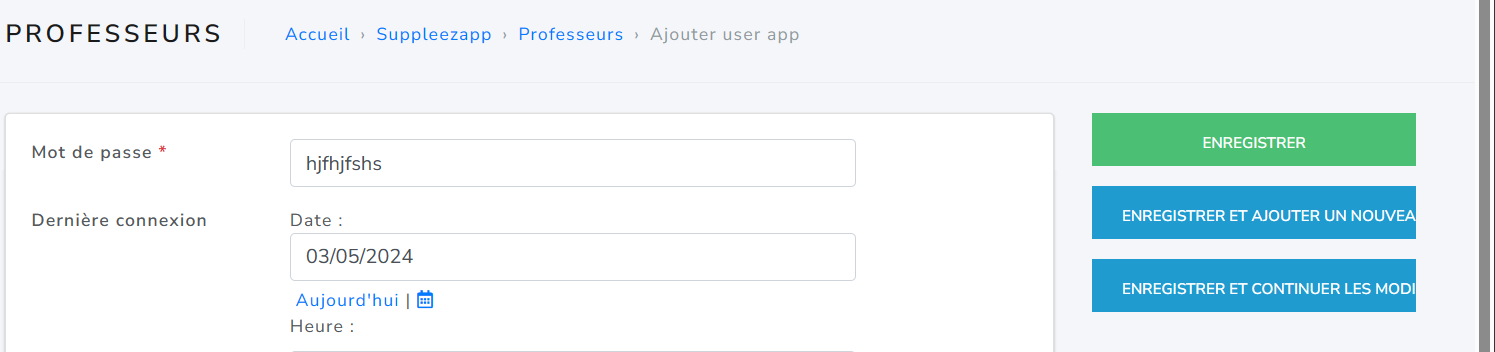
\includegraphics[width=0.75\linewidth]{image42.png}
    \caption{Adding a Professor - Final Step}
\end{figure}

\subsubsection{Creating a Request}\label{12}

To create a request, proceed as follows:

\begin{enumerate}
    \item Begin by selecting the professor for whom you want to create the request.
    \item Next, choose the course for which the request is being made.
    \item Specify whether the course is optional or not.
    \item Enter the reason for the request and select the salary allocation option.
    \item If necessary, fill in additional fields such as the CPO number and supervisor agreement.
    \item Choose the status of the request (e.g., "En cours de traitement," "Approuvé," or "refusé").
    \item Finally, click on the "Save" button at the top of the page to submit the request.
\end{enumerate}

\begin{figure}[H]
    \centering
    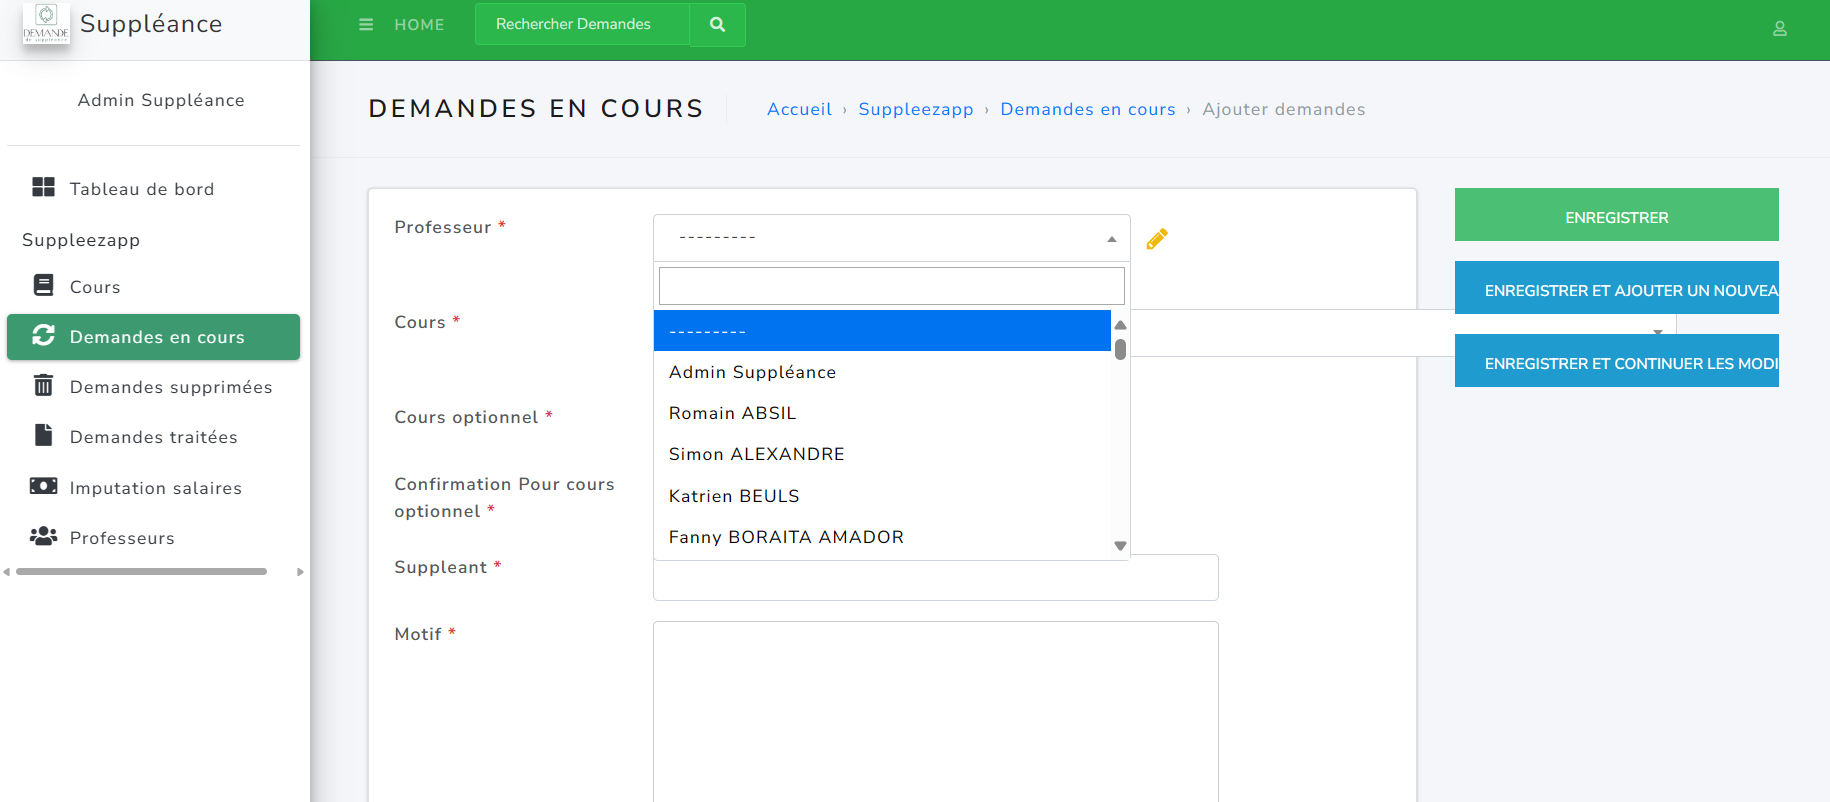
\includegraphics[width=0.75\linewidth]{image45.png}
    \caption{Selecting Professor for Request}
\end{figure}

\begin{figure}[H]
    \centering
    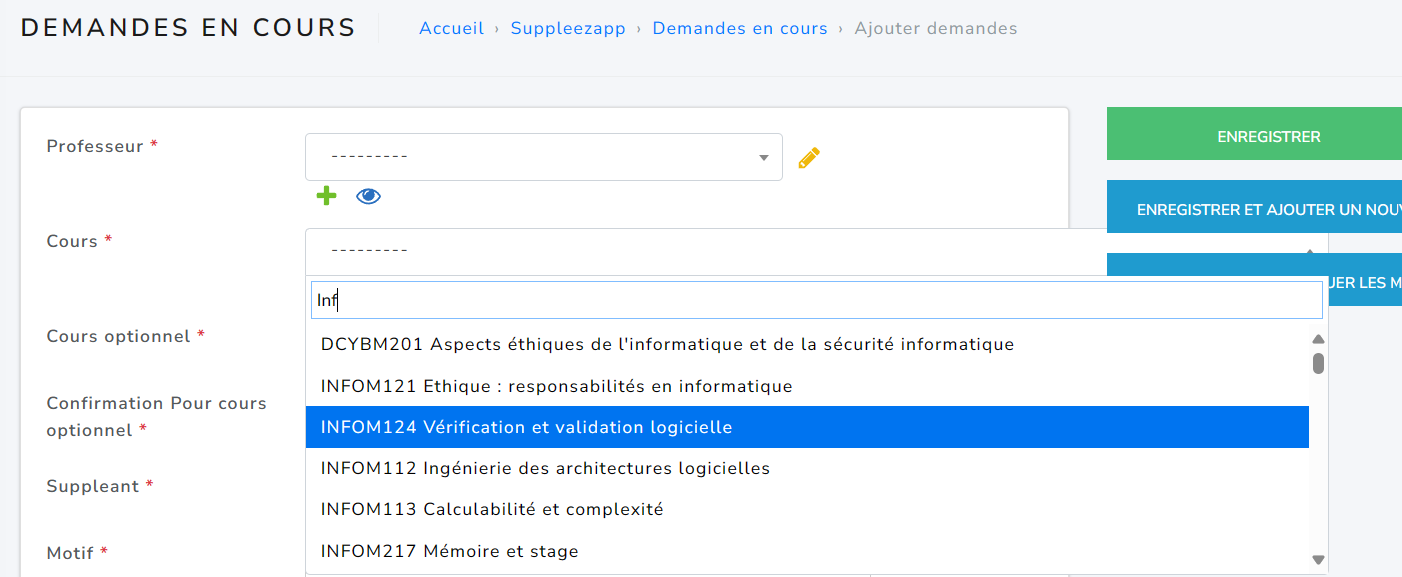
\includegraphics[width=0.75\linewidth]{image50.png}
    \caption{Choosing Course for Request}
\end{figure}

\begin{figure}[H]
    \centering
    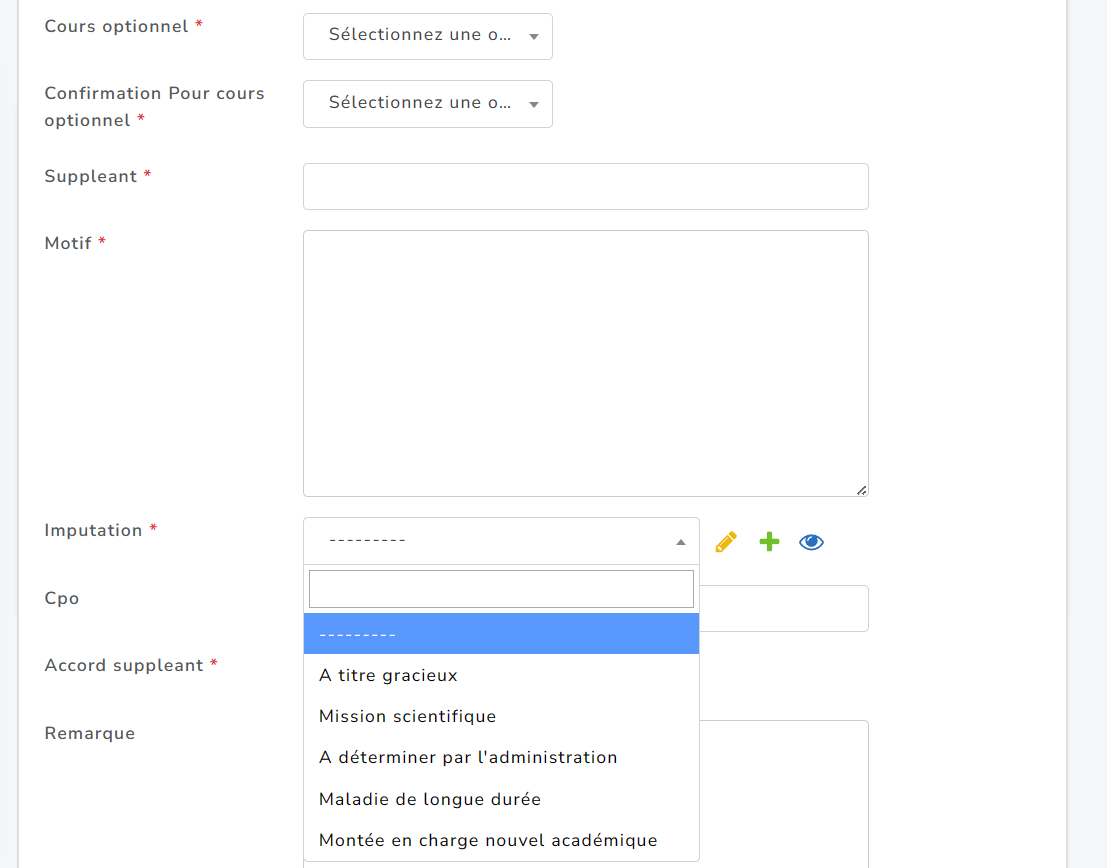
\includegraphics[width=0.75\linewidth]{image51.png}
    \caption{Entering Request Details}
\end{figure}

\begin{figure}[H]
    \centering
    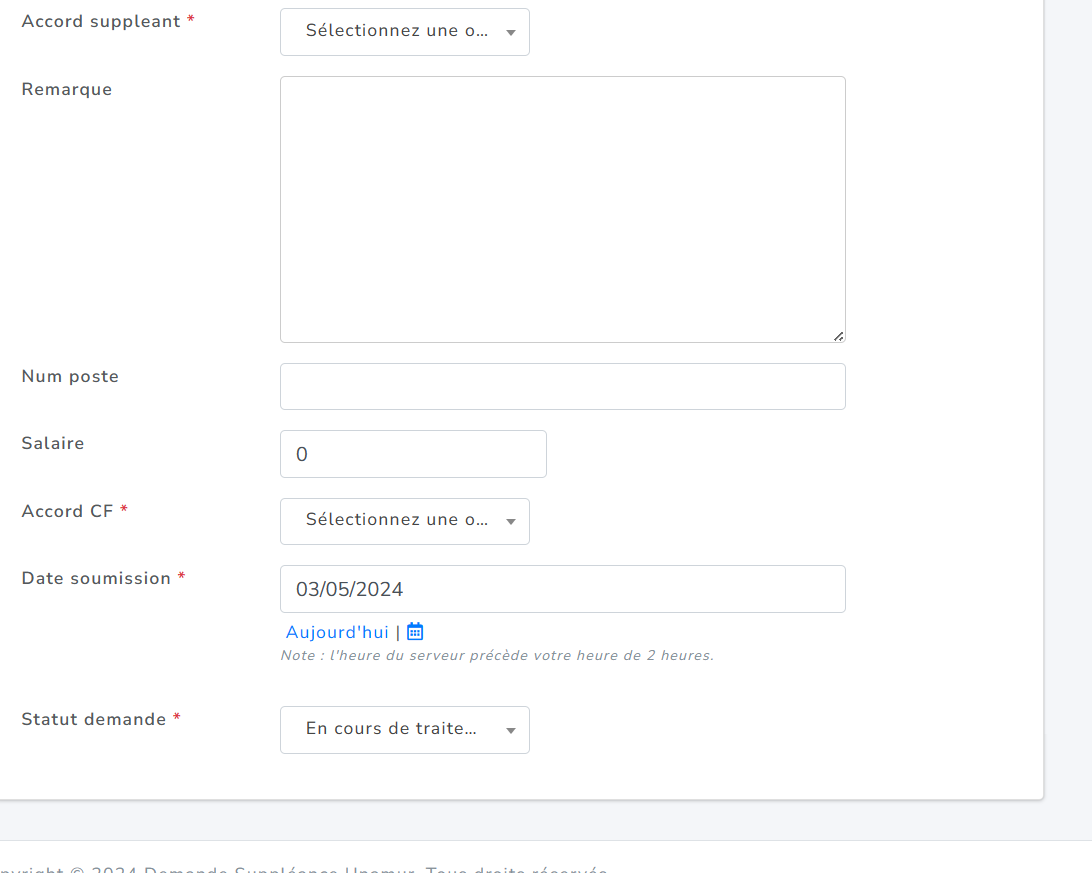
\includegraphics[width=0.75\linewidth]{image52.png}
    \caption{Specifying Request Status}
\end{figure}

\begin{figure}[H]
    \centering
    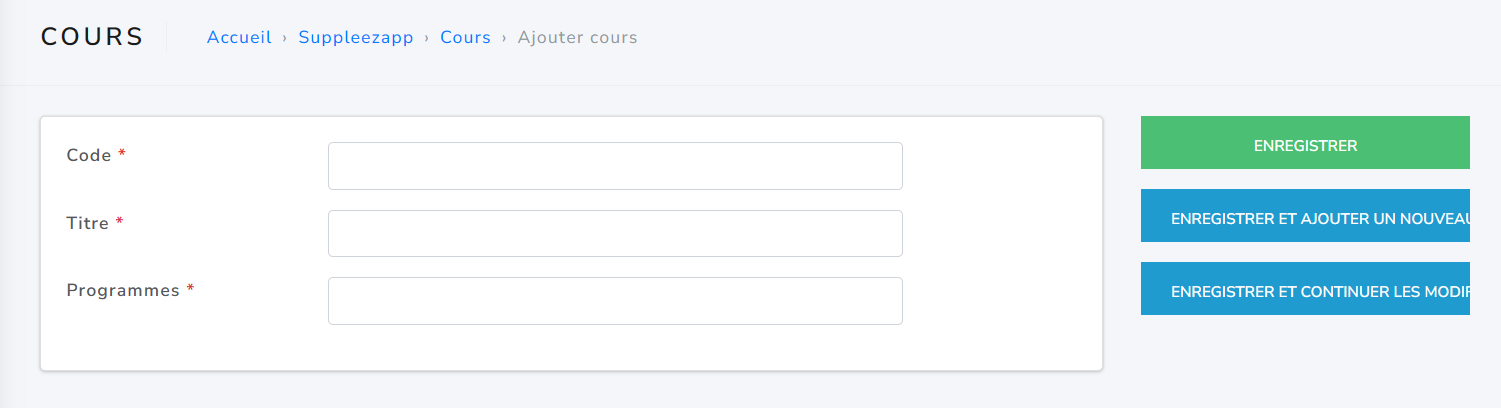
\includegraphics[width=0.75\linewidth]{image54.png}
    \caption{Saving the Request}
\end{figure}

\subsubsection{Adding a Course}

To add a new course, follow these steps:

\begin{enumerate}\label{13}
    \item Access the section for adding courses.
    \item Fill in all the required information for the course, including its name, code, and any additional details.
    \item Once all information is entered, click on the "Enregistrer" button to add the course to the system.
\end{enumerate}

\begin{figure}[H]
    \centering
    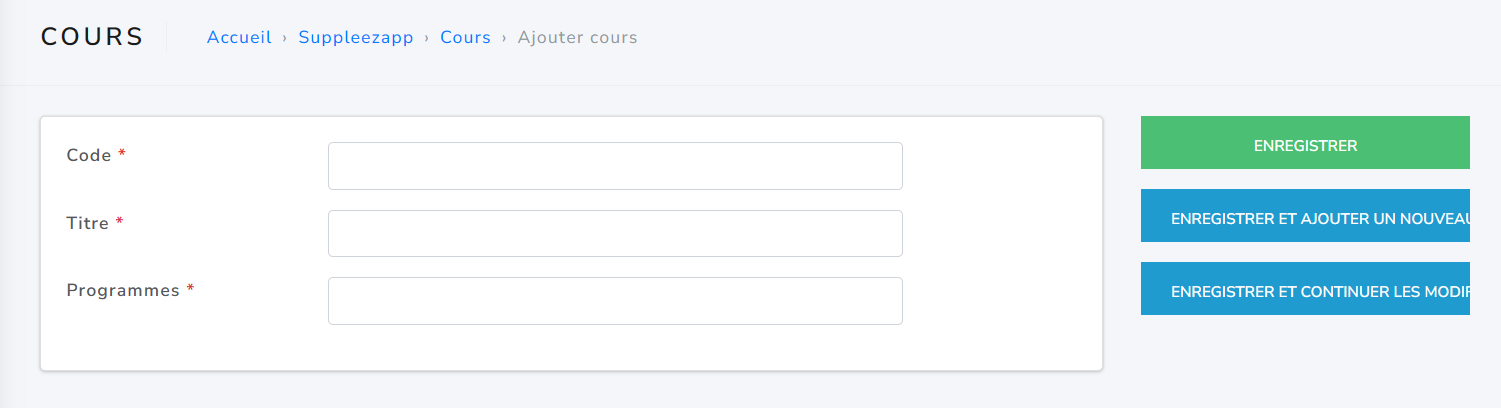
\includegraphics[width=0.75\linewidth]{image54.png}
    \caption{Adding a Course}
\end{figure}

\subsection{Modifying Existing Entries}

To modify any existing entry, whether it's a course, professor, request, or salary allocation, follow these general steps:

\begin{enumerate}
    \item Navigate to the respective table or section containing the entry you wish to modify.
    \item Click on the specific element within the table representing the entry you want to modify.
    \item A page containing a form with the information of the selected element will appear.
    \item Make the necessary modifications to the information.
    \item Once you have made the desired changes, click on the "Enregistrer" button to save the modifications.
\end{enumerate}

This process applies universally to modifying any type of entry within the application.
\subsection{How to Modify Password and Profile}

Clicking on the icon at the top right corner of the dashboard provides options to modify the password and view/edit the profile details.

\begin{figure}[H]
    \centering
    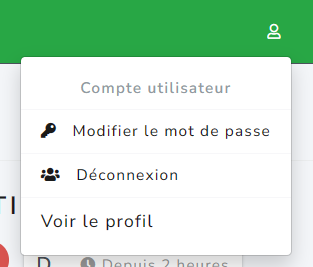
\includegraphics[width=0.5\linewidth]{image55.png}
    \caption{Modify Password and Profile}
\end{figure}

To modify the password, fill in the old password, new password, and click on "Modifier le Mot de Passe." Similarly, you can access and edit the profile details from the "Profile" option. illustrations below:

\begin{figure}[H]
    \centering
    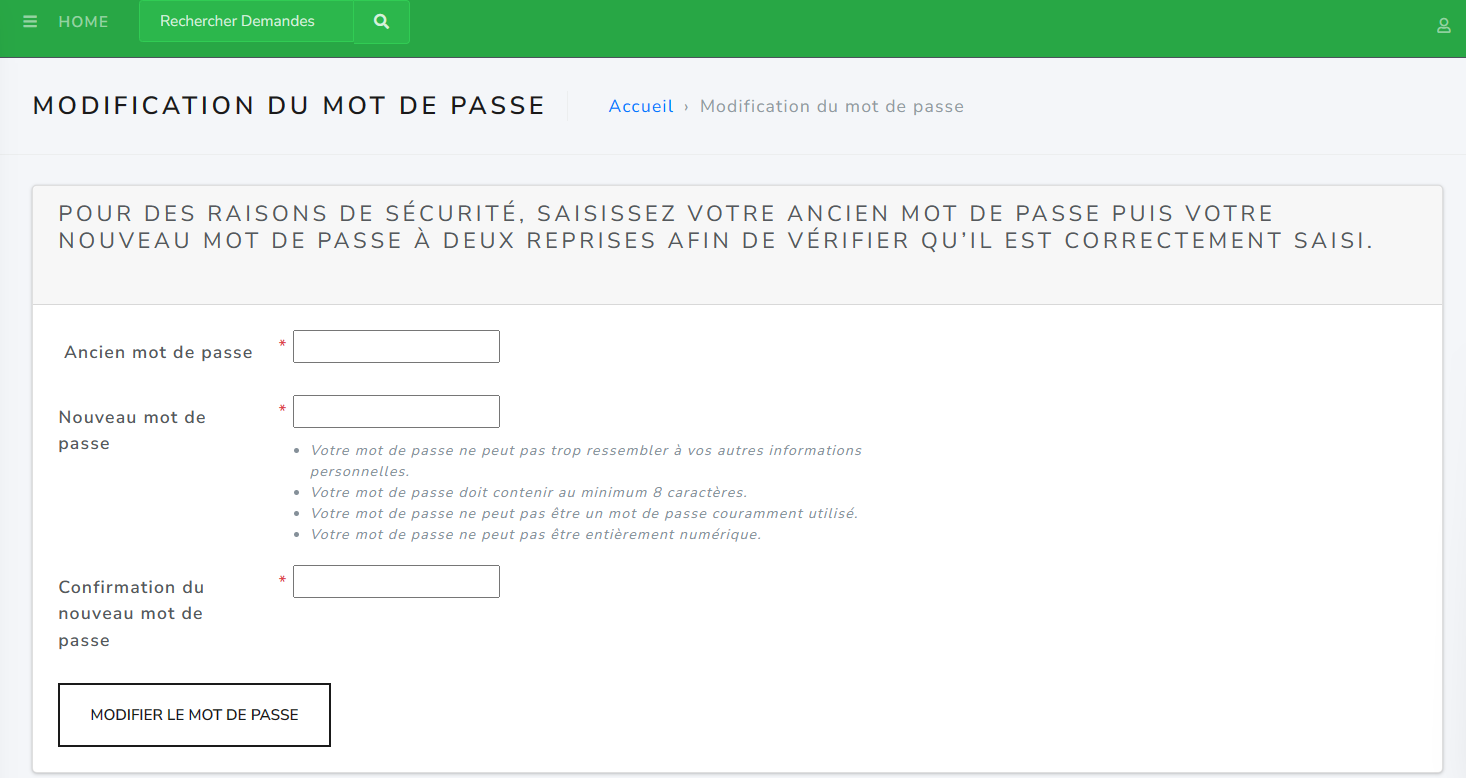
\includegraphics[width=0.75\linewidth]{image56.png}
    \caption{Modify Password Page}
\end{figure}

\begin{figure}[H]
    \centering
    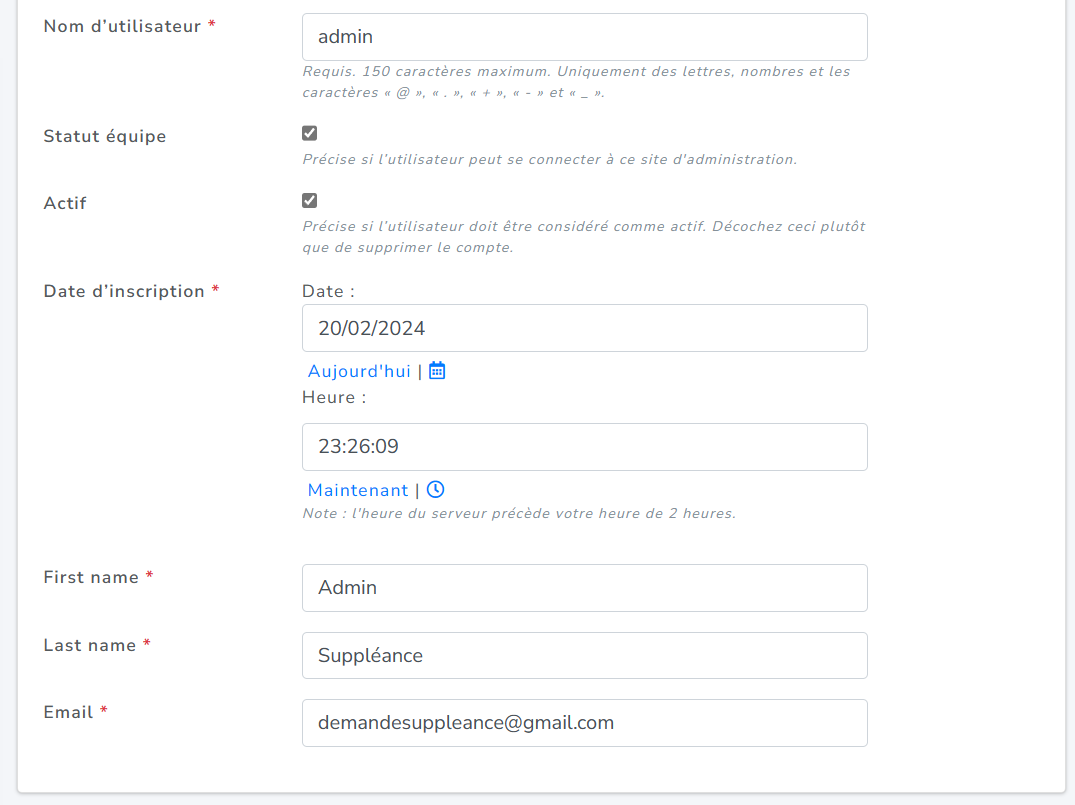
\includegraphics[width=0.75\linewidth]{image57.png}
    \caption{Profile Page}
\end{figure}

Finally, the "Déconnexion" button logs you out of the application and returns you to the site's home page.
\section{Troubleshooting / FAQ}\label{trouble}

\subsection{Unable to Log In}

\textbf{Problem:} Users are unable to log in to the application.

\textbf{Solution:}
\begin{enumerate}
    \item \textbf{Check Credentials:} Ensure that the username and password entered are correct. Pay attention to uppercase and lowercase letters.
    \item \textbf{Reset Password:} If the password is forgotten, use the "Mot de passe oublié?" feature to reset it. Follow the instructions sent to the registered email address.
    \item \textbf{Network Connection:} Verify that the device has a stable internet connection. Try connecting to a different network if possible.
\end{enumerate}

\subsection{Error Messages}

\textbf{Problem:} Users encounter error messages while using the application.

\textbf{Solution:}
\begin{enumerate}
    \item \textbf{Read Error Message:} Carefully read the error message displayed on the screen. It may provide information about the issue.
 
    \item \textbf{Contact Support:} If the error persists or is unclear, contact the application support team for assistance. Provide detailed information about the error message and steps to reproduce the issue.
\end{enumerate}

\subsection{Slow Performance}

\textbf{Problem:} The application is running slowly or experiencing delays.

\textbf{Solution:}
\begin{enumerate}
    \item \textbf{Device Performance:}  Close any unnecessary applications running in the background.
    \item \textbf{Network Speed:} Verify the internet connection speed. A slow network connection can affect application performance. Consider switching to a faster network if available.
    \item \textbf{Clear Cache:} Clear the application cache to remove temporary files that may be causing slowdowns. This option is usually found in the application settings.
\end{enumerate}

\subsection{Data Sync Issues}

\textbf{Problem:} Data synchronization problems between devices or servers.

\textbf{Solution:}
\begin{enumerate}
    \item \textbf{Refresh Data:} Try refreshing the application or reloading the page to force a synchronization attempt.

    \item \textbf{Sync Settings:}  Adjust settings as needed to resolve synchronization conflicts.
\end{enumerate}

\subsection{Feature Not Working}

\textbf{Problem:} A specific feature of the application is not functioning as expected.

\textbf{Solution:}
\begin{enumerate}
    \item \textbf{Check Updates:} Verify that the application is up to date. Updates may include bug fixes or enhancements to resolve issues with specific features.
    \item \textbf{Restart Application:} Close and reopen the application to refresh its state. Sometimes, this simple action can resolve minor issues.
    \item \textbf{Report Bug:} If the feature continues to malfunction, report the issue to the application developers or support team. Provide detailed information about the feature and steps to reproduce the problem for faster resolution.
\end{enumerate}

\section{Contact}

For any inquiries or suggestions, please feel free to contact us via email at ulrich.toujinana@student.unamur.be or ulrich.nana90@gmail.com.

\end{document}


